\chapter{Transcodificação de Vídeo Baseado em Aprendizado de Máquina}
\label{cap:7}

Ao longo do texto, apresentamos o uso de aprendizado de máquina como uma importante estratégia para tornar as propostas de aceleração da transcodificação mais eficientes. Como foi ressaltado no capítulo \ref{cap:3}, trabalhos envolvendo aprendizado de máquina tendem a apresentar resultados mais satisfatórios de TS e BD-rate do que aqueles baseados em análises estatísticas. Apesar dos resultados de propostas baseadas em aprendizado de máquina serem positivos, a adaptação das estratégias em outros transcodificadores rápidos é algo incomum, principalmente em transcodificações heterogêneas, já que pode ser difícil, ou mesmo impossível, compatibilizar as complexas ferramentas de diferentes formatos de codificação de vídeo. Portanto, um dos objetivos apresentados neste capítulo é desenvolver um \textit{pipeline} de processamento que possibilite a adaptação da metodologia de desenvolvimento de transcodificadores rápidos para diversas combinações de formatos utilizando aprendizado de máquina. Embora abordemos especificamente o algoritmo de aprendizado de máquina CART (veja seção \ref{cap:7.1}), a alteração de algoritmos e/ou de seus hiperparâmetros, dentro do \textit{pipeline}, é simples e intuitiva.

Para fins de viabilidade e prova de conceito do \textit{pipeline} de processamento proposto, este capítulo apresenta soluções geradas para transcodificadores de diversos formatos para o formato AV1, adaptando um trabalho original desenvolvido de VP9 para AV1. Contudo, ao invés de apresentar múltiplas soluções distintas, ou seja, um transcodificador rápido para cada combinação de formatos (como os apresentados no capítulo \ref{cap:6}), este capítulo propõe a aplicação do \textit{pipeline} proposto, a fim de permitir a geração de soluções para os vários transcodificadores rápidos de forma simplificada.

Como descrito no capítulo \ref{cap:3}, o reaproveitamento de estruturas de particionamento de blocos é uma das principais abordagens em trabalhos de transcodificador rápido observados na literatura científica. Uma das principais razões dessa relevância está no fato de que o número de tamanhos de blocos avaliados está diretamente relacionados com a alta complexidade das predições intraquadro e interquadros, inclusive das transformadas, já que a busca pelos melhores modos preditivos se dá pela busca (por vezes exaustiva) dos diversos tamanhos de blocos disponíveis. Logo, reduzir a quantidade de tamanhos de bloco a serem considerados na recodificação do vídeo reduz consideravelmente a complexidade do codificador. No capítulo \ref{cap:5}, abordamos o impacto na eficiência da codificação do AV1 ao manipular a sua árvore de particionamentos. Portanto, as soluções desenvolvidas para transcodificação rápida usando modelos preditivos gerados por algoritmos de aprendizado de máquina, descritas neste capítulo da tese, possuem como base o treinamento de modelos com o objetivo de predizer o particionamento do bloco em quatro novos ramos.

Assim, apresentamos dois desafios neste capítulo: (1) verificar a possibilidade de implementar um \textit{pipeline} de processamento que permita a adaptação de soluções para transcodificadores rápidos de forma simplificada e escalonável, ou seja, se é possível utilizar os mesmos passos empregados no desenvolvimento de um transcodificador rápido ao desenvolver um outro transcodificador rápido para outra combinação de formatos; e (2) averiguar se o \textit{pipeline} permite atingir resultados compatíveis com o observado na literatura, independentemente da combinação de formatos utilizados como fonte e destino. 

As soluções para aceleração de transcodificadores geradas a partir do \textit{pipeline} proposto baseiam-se nos formatos mais comuns na indústria de \textit{streaming} da atualidade, conforme \citet{bib:bitmovin_report_2021} e \citet{bib:bitmovin_report_2022}: H.264/AVC, H.265/HEVC, VP9, VP8, VVC e AV1. Como deve ter ficado evidente até este momento, optamos por utilizar  o AV1 como formato de destino.

Além do nosso trabalho apresentado na seção \ref{cap:5.2}, não existem outros trabalhos conhecidos com foco na aceleração da transcodificação de VP9 para AV1. Há na literatura alguns trabalhos de transcodificação rápida de H.265/HEVC para AV1, vide \citet{bib:borges_2019}, \citet{bib:borges2_2019}, \citet{bib:borges2_2021} e \citet{bib:chen_2019}. Inclusive, os autores deste último desenvolveram uma solução envolvendo aprendizado de máquina (trabalho já abordado nas seções \ref{cap:3.1} e \ref{cap:6.1}). As demais soluções transcodificação que adaptamos por meio do uso de nosso \textit{pipeline} são de transcodificações rápidas inéditas, até o presente momento, na literatura: VP8-para-AV1, H.264/AVC-para-AV1 e H.266/VVC-para-AV1.

Conforme discutido no capítulo \ref{cap:1} com base no relatório publicado por \citet{bib:bitmovin_report_2021} e \citet{bib:bitmovin_report_2022}, os formatos listados (H.264/AVC, H.265/HEVC, VP9 e VP8) são os mais utilizados na indústria de \textit{streaming} de vídeos. Portanto, apresentamos soluções para aceleração de transcodificação para o formato de codificação de vídeo AV1 a partir de praticamente 100\% dos formatos utilizados no mercado internacional de streaming de vídeo, com exceção da China, que utiliza formatos próprios \cite{bib:china_codecs}.

Assim exposto, este capítulo apresenta as seguintes contribuições nas próximas seções:

\begin{enumerate}[1.]
    \item Um \textit{pipeline} de processamento para geração de soluções de transcodificadores rápidos de vídeo com uso de modelos preditivos treinados através de aprendizado de máquina;

    \item Um transcodificador VP9-para-AV1, acelerado através do uso de árvores de decisão;

    \item Um transcodificador H.264/AVC-para-AV1, acelerado através do uso de árvores de decisão;

    \item Um transcodificador H.265/HEVC-para-AV1, acelerado através do uso de árvores de decisão;

    \item Um transcodificador VP8-para-AV1, acelerado através do uso de árvores de decisão;

    \item Um transcodificador H.266/VVC-para-AV1, acelerado através do uso de árvores de decisão.
    
\end{enumerate}

Para permitir o desenvolvimento e a prova de conceito do \textit{pipeline} de processamento proposto, algumas decisões precisaram ser tomadas, descritas na seção \ref{cap:7.1}. A seção \ref{cap:7.2} se dedica a abordar o funcionamento do \textit{pipeline} proposto e suas fases de execução automatizadas. Os detalhes mais importantes desse \textit{pipeline} de processamento são aprofundados nas seções \ref{cap:7.3} (seleção dos modelos de aprendizado de máquina) e \ref{cap:7.4} (algoritmo de transcodificação a ser adaptado pelas propostas).

\section{Metodologia e Ferramental Utilizado}
\label{cap:7.1}

Apesar de os vídeos de ultra alta definição estarem crescendo em uso, principalmente UHD4K (de 3840$\times$2160 ou 4096$\times$2160 pixels), é a resolução de alta-definição 1080 (HD1080, de 1920$\times$1080 pixels) que é a mais consumida pelos usuários de serviços de \textit{streaming} \cite{bib:bitmovin_twitter}. Portanto, nas soluções desenvolvidas neste capítulo, dedicamos esforços para apresentar resultados nessa categoria de vídeos, mais especificamente em sequências de vídeo naturais HD1080. No entanto, sequências de vídeos naturais HD720 e UHD4K também serão consideradas, sempre que possível, para avaliação dos modelos preditivos. É importante destacar que, como qualquer outro trabalho envolvendo aprendizado de máquina, os conjuntos de dados precisam ser divididos em três subconjuntos, conforme discutido na seção \ref{cap:2.2}: de treinamento, de teste e de predição. Visando construir um vasto conjunto de vídeos, independentes entre si, utilizamos todos os vídeos HD1080 disponíveis nas condições comuns de teste dos documentos \cite{bib:av2_avm}, \citet{bib:hevcctc} e \citet{bib:ietfnetvct}, para compor, respectivamente, os conjuntos de treino (sete sequências), de teste (sete sequências) e de predição (demais sequências). Como pode ser visto na Tabela \ref{tab:XVII}, fazem parte dos vídeos de predição 48 sequências, distribuídas entre as resoluções HD720, HD1080 e UHD4K. Como foi dito no capítulo \ref{cap:4}, o Apêndice \ref{apx:A} descreve com detalhes as sequências utilizadas. Na Tabela \ref{tab:XVII}, constam os nomes das sequências utilizadas em cada uma das fases de desenvolvimento das soluções propostas neste capítulo.

\begin{table}
\begin{center}
\caption{Sequências de vídeo selecionadas para compor os conjuntos dos experimentos.}
\label{tab:XVII}
\footnotesize

\begin{tblr}{
    colspec = {l|p{13cm}},
    hlines,
    row{even} = {gray9}
}
\hline
\textbf{Fase} & \textbf{Sequências}  \\
Treinamento & BasketballDrive\_1920x1080\_50, BQTerrace\_1920x1080\_60, Cactus\_1920x1080\_50, CrowdRun\_1920x1080\_25, Kimono1\_1920x1080\_24, ParkScene\_1920x1080\_24, Tennis\_1920x1080\_24 \\
Teste        & FountainSky\_1920x1080p30\_130f, TimeLapseStreet\_1920x1080p30\_130f, Wheat\_1920x1080, WorldCup\_1920x1080\_30p, WorldCup\_far\_1920x1080\_30p, WorldCupFarSky\_1920x1080\_30p, Skater227\_1920x1080\_30fps \\
Predição    & aspen\_1080p\_60f, crowd\_run\_1080p50\_60f, dark720p\_120f, ducks\_take\_off\_1080p50\_60f, FourPeople\_1280x720\_60, FourPeople\_1280x720\_60\_120f, gipsrestat720p\_120f, Johnny\_1280x720\_60, Johnny\_1280x720\_60\_120f, KristenAndSara\_1280x720\_60, KristenAndSara\_1280x720\_60\_120f, Netflix\_Aerial\_1920x1080\_60fps\_8bit\_420\_60f, Netflix\_Boat\_1920x1080\_60fps\_8bit\_420\_60f, Netflix\_Crosswalk\_1920x1080\_60fps\_ 8bit\_420\_60f, Netflix\_DinnerScene\_1280x720\_60fps\_8bit\_420\_120f, Netflix\_DrivingPOV\_1280x720\_60fps\_8bit\_420\_120f, Netflix\_FoodMarket\_1920x1080\_60fps\_8bit\_420\_60f, Netflix\_FoodMarket2\_1280x720\_60fps\_8bit\_420\_120f, Netflix\_PierSeaside\_1920x1080\_60fps\_8bit\_420\_60f, Netflix\_RollerCoaster\_1280x720\_60fps\_8bit\_420\_120f, Netflix\_SquareAndTimelapse\_1920x1080\_60fps\_8bit\_420\_60f, Netflix\_Tango\_1280x720\_60fps\_8bit\_420\_120f, Netflix\_TunnelFlag\_1920x1080\_60fps\_8bit\_420\_60f, old\_town\_cross\_1080p50\_60f, park\_joy\_1080p50\_60f, pedestrian\_area\_1080p25\_60f, rush\_field\_cuts\_1080p\_60f, rush\_hour\_1080p25\_60f, station2\_1080p25\_60f, Vidyo1\_1280x720\_60, vidyo1\_720p\_60fps\_120f, Vidyo3\_1280x720\_60, vidyo3\_720p\_60fps\_120f, Vidyo4\_1280x720\_60, vidyo4\_720p\_60fps\_120f, boat\_hdr\_amazon\_720p, guitar\_hdr\_amazon\_1080p, pan\_hdr\_amazon\_1080p, rain\_hdr\_amazon\_720p, seaplane\_hdr\_amazon\_1080p, Netflix\_BarScene\_4096x2160\_60fps\_10bit\_420\_60f, Netflix\_BoxingPractice\_4096x2160\_60fps\_10bit\_420\_60f, Netflix\_Dancers\_4096x2160\_60fps\_10bit\_420\_60f, Netflix\_Narrator\_4096x2160\_60fps\_10bit\_420\_60f, Netflix\_RitualDance\_4096x2160\_60fps\_10bit\_420\_60f, Netflix\_ToddlerFountain\_4096x2160\_60fps\_10bit\_420\_60f, Netflix\_WindAndNature\_4096x2160\_60fps\_10bit\_420\_60f, street\_hdr\_amazon\_2160p \\
\hline
\end{tblr}
\end{center}
\end{table}


\subsection{Algoritmos de Aprendizado de Máquina}
\label{cap:7.1.3}

No capítulo \ref{cap:4}, especificamos que a linguagem Python versão 3 foi utilizada para o desenvolvimento de algumas soluções apresentadas nesta tese, em particular as apresentadas no atual capítulo. Dentre essas soluções, está o treinamento de modelos preditivos gerados por algoritmos de aprendizado de máquina. Existem diversas ferramentas, desenvolvidas em Python, que possibilitam essa geração de modelos preditivos, dentre elas o pacote \textit{Scikit-Learn} \cite{bib:scikitlearn-site}. Esse pacote oferece um algoritmo para treinamento de árvores de decisão que permitem a classificação e a regressão de valores, denominado \textit{Classification and Regression Trees} (CART) \cite{bib:scikitlearn_cart}, baseado no trabalho de \citet{bib:livroCART}. Este algoritmo permite a manipulação de alguns hiperparâmetros, descritos na Tabela \ref{tab:XVIII}. Nesta tabela apresentamos os hiperparâmetros existentes no algoritmo CART e seus respectivos valores usados nas soluções propostas de transcodificação rápida com uso de modelos gerados pelo algoritmo CART. Na última coluna da Tabela \ref{tab:XVIII}, apresentamos a quantidade de variações existentes para cada hiperparâmetro, considerando os valores que utilizaremos. Logo, calculando-se o produto dessas variações, há um total de 9,5 milhões de modelos candidatos de aprendizado de máquina a serem treinados com este algoritmo. Observe que, em vários hiperparâmetros da Tabela \ref{tab:XVIII} que utilizam valores inteiros como entrada, consideramos um valor máximo de 25. A razão disso é a quantidade de atributos utilizados nos trabalhos deste capítulo, que é de 25, conforme consta na seção \ref{cap:7.3}.

\afterpage{
\clearpage

\begin{landscape}
{\footnotesize
\begin{longtblr}[
    caption = {Relação dos hiperparâmetros disponíveis no algoritmo CART.},
    label = {tab:XVIII}
]{
    colspec = {l|p{14cm}|p{4.2cm}|r},
    rowhead = 1,
    hlines,
    row{even} = {gray9}
}
\hline
\textbf{Hiperparâmetro} & \textbf{Descrição} & \textbf{Valores Utilizados} & \textbf{Quantidade} \\
\textit{Criterion} & Define a função para medir a qualidade do subparticionamento árvore de decisão. Podem ser utilizados ganho de impureza gini ou ganho de informação por entropia de Shannon, conforme descritos em \citet{bib:CART_matematica}. & 'gini', 'entropy' & 2 \\
\textit{Splitter} & Define a estratégia utilizada para escolher o subparticionamento em cada nó da árvore de decisão. É possível optar pela melhor divisão ou divisão aleatória. & 'best', 'random' & 2 \\
\textit{Max Depth} & Define a profundidade máxima da árvore de decisão. O valor ‘None’ indica que não há um limite definido. & 'None', 3, 5, 7, 11, 13, 17, 19, 25 & 9 \\
\textit{Min Samples Split} & Define o número mínimo de amostras necessárias para subparticionar um nó interno (no mínimo duas amostras). & 2, 3, 5, 7, 11, 13, 17, 19, 25 & 9 \\
\textit{Min Samples Leaf} & Define o número mínimo de amostras necessárias para tornar um nó como folha. Ou seja, o subparticionamento em qualquer profundidade só será considerado se, pelo menos este número de amostras, estiver tanto no ramo do lado esquerdo como no lado direito.  & 1, 3, 5, 7, 11, 13, 17, 19, 25 & 9 \\
\textit{Max Features} & Define o número de atributos a serem considerados ao procurar o melhor subparticionamento do nó. Pode ser a raiz quadrada, ou o logaritmo de base dois da quantidade de atributos disponíveis, ou nenhum, indicando que todos os atributos devem ser utilizados. & 'sqrt', 'log2', 'None' & 3 \\
\textit{Max Leaf Nodes} & Define o número máximo de nós folhas. Em caso de ‘None’, não há limite máximo. A escolha pelos melhores nós é definida pelo próximo atributo. & 'None', 3, 5, 7, 11, 13, 17, 19, 25 & 9 \\
\textit{Min Impurity Decrease} & Define se um nó deve ser subparticionamento ou não, caso esta divisão induza a uma diminuição na impureza maior ou igual ao valor definido. & 0,0, 0,1, 0,2, 0,3, 0,4, 0,5, 0,6, 0,7, 0,8, 0,9, 1,0 & 11 \\
\textit{CPP Alpha} & Define o valor a ser usado para poda antecipada considerando a mínima taxa entre custo e complexidade (\textit{Minimal Cost-Complexity Pruning}, conforme \citet{bib:CART_cppalpha}). A subárvore com uma taxa inferior ao definido será escolhida. Se 0.0, nenhuma poda é executada. & 0,0, 0,1, 0,2, 0,3, 0,4, 0,5, 0,6, 0,7, 0,8, 0,9, 1,0 & 11 \\
\SetCell[c=3]{r}Quantidade Total de Modelos &&& 9.526.572 \\
\hline
\end{longtblr}
}
\end{landscape}
}


\subsection{Mensuração de Resultados}
\label{cap:7.1.4}

Na seção \ref{cap:2.4} discutimos as métricas estatísticas \textit{F1-Score} (Equação \ref{eq:6}) e AUC (Figura \ref{fig:8}) para avaliação dos treinamentos dos modelos preditivos gerados por algoritmos de aprendizado de máquina. O pacote \textit{scikit-learn} oferece meios de mensurar essas métricas, por meio do módulo ``\textit{sklearn.metrics}'', que permite utilizar as funções ``\textit{f1\_score}'' \cite{bib:scikitlearn_f1} e ``\textit{roc\_auc\_score}'' \cite{bib:scikitlearn_auc}. Essas duas funções possuem diversos parâmetros de utilização, conforme pode ser observado em documentação própria \cite{bib:scikitlearn_f1, bib:scikitlearn_auc}. Serão utilizados os valores padrões dessas funções, exceto por um único parâmetro: ``\textit{average}''. Por padrão, esse parâmetro avalia apenas os resultados positivos preditos pelo modelo treinado; no entanto, apesar dos modelos treinados pelas nossas propostas terem rótulos binários (ver mais na seção \ref{cap:7.3}), a relevância das respostas positivas tanto quanto as negativas possuem igual importância. Dessa forma, como é importante que as funções ``\textit{f1\_score}'' e ``\textit{roc\_auc\_score}'' avaliem ambas respostas do rótulo igualmente, o parâmetro ``\textit{average}'' deve ser configurado como ``\texttt{macro}''.

Em relação às métricas para comparação dos resultados de transcodificação rápida, empregamos os valores de TS (Equação \ref{eq:7}) e de BD-rate (Figura \ref{fig:9}), ambos já apresentados na seção \ref{cap:2.5}. Em relação à captura do tempo de processamento, valor importante para gerar o TS, usamos os valores informados pelo próprio software de referência do AV1, cujo tempo total da codificação é mensurado em milissegundos, posteriormente convertidos para segundos. Já no caso do BD-rate, utilizamos os valores de bitrate (em kilobits por segundo, kbps) e de PSNR-Y (em decibéis, dB).

\section{Visão Geral do \textit{Pipeline} de Processamento}
\label{cap:7.2}

O \textit{pipeline} de processamento proposto para o desenvolvimento das soluções baseadas em aprendizado de máquina está representado, em alto nível, pela Figura \ref{fig:25}, sendo notória a existência de quatro fases de execução. Cada uma dessas fases é descrita nas subseções a seguir, mas todas elas compartilham das mesmas configurações gerais. O compartilhamento dessas configurações permite que as quatro fases mantenham uma sincronia em relação a variáveis como as sequências de vídeo a serem utilizadas, núcleos de processamento autorizados para uso, arquivos a serem substituídos nos softwares de referência, identificações e meios de compilação desses softwares, lista de configurações dos hiperparâmetros do algoritmo de aprendizado de máquina, entre outros valores. Essa centralização de configurações facilita a realização de modificações rápidas nos experimentos, garantindo uma maior agilidade e confiabilidade no \textit{pipeline}.

\begin{figure}
    \centering
    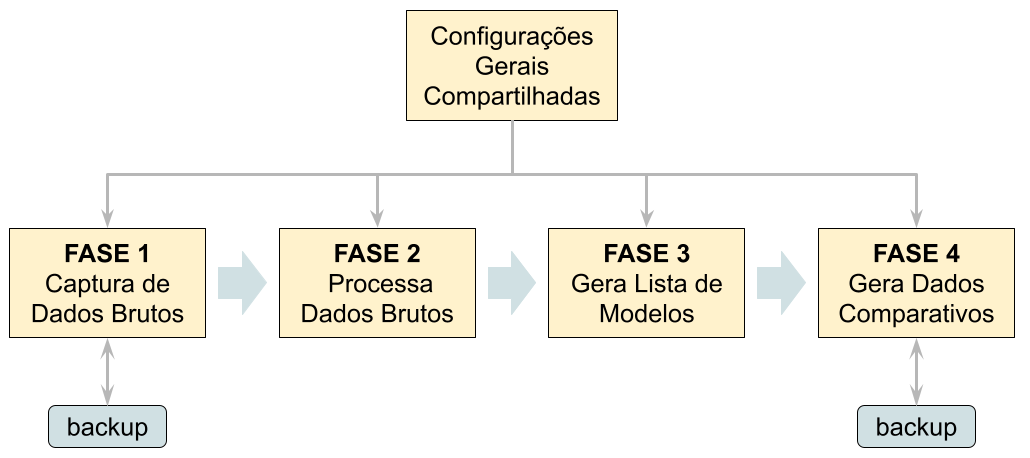
\includegraphics[width=\textwidth]{FIGURES/fig_25.png}
    \caption{Representação em alto nível do fluxo de execução do \textit{pipeline} de processamento. Fonte: Elaborada pelo autor.}
    \label{fig:25}
\end{figure}

Após a configuração geral do experimento e dos softwares, conforme descrito na seção \ref{cap:4.2}, o \textit{pipeline} automatiza a execução de todas as quatro fases. Nas Fases 1 e 4, um sistema de backup auxilia a retomada dos experimentos em caso de interrupção. A Fase 3 é responsável pela seleção do melhor modelo de aprendizado de máquina treinado com os dados gerados da Fase 2.

O algoritmo implementado no transcodificador rápido de VP9-para-AV1, e que será adaptado para os demais formatos considerados neste capítulo, será utilizado nas Fases 1, 2 e 4. Esse algoritmo será descrito com detalhes na seção \ref{cap:7.4}. Enquanto a seleção do melhor modelo de aprendizado de máquina (Fase 3) é descrita na seção \ref{cap:7.3}. O código-fonte do \textit{pipeline} proposto está disponível em \citet{bib:prototipotese}.

\subsection{Fase 1: Captura de Dados Brutos}
\label{cap:7.2.1}

É responsabilidade desta fase a captura dos dados brutos para treinamento e teste dos modelos de aprendizado de máquina. Os vídeos codificados no antigo formato são decodificados, gerando dois arquivos: o vídeo decodificado e os dados extraídos durante a decodificação. A partir do vídeo decodificado, a transcodificação é concluída com uma recodificação do conteúdo no novo formato, sem qualquer processo de aceleração, exportando um conjunto de dados. O fluxo de execução da Fase 1 é demonstrado na Figura \ref{fig:26}. Em todas as soluções apresentadas neste capítulo, o codificador utilizado foi o software \textit{libaom} do AV1. De forma geral, esta fase é responsável por:

\begin{enumerate}[1.]
    \item Decodificar o \textit{bitstream} pertencente ao conjunto de treinamento e de teste, que foi codificado em um formato pré-definido;

    \item Exportar informações provenientes do decodificador;

    \item Recodificar o vídeo decodificado para o novo formato, utilizando parâmetros de quantização pré-definidos;

    \item Exportar informações provenientes do codificador.
\end{enumerate}

\begin{figure}
    \centering
    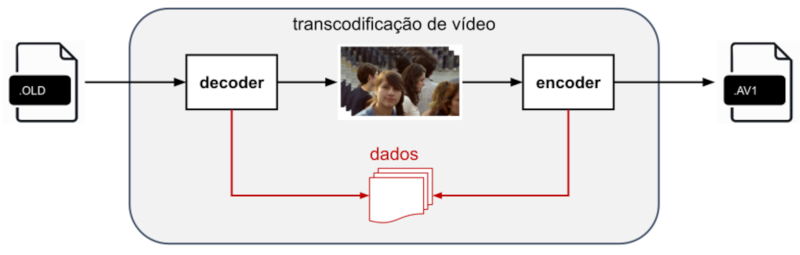
\includegraphics[width=0.85\textwidth]{FIGURES/fig_26.png}
    \caption{Representação da transcodificação realizada na Fase 1. Fonte: Elaborada pelo autor.}
    \label{fig:26}
\end{figure}


\subsection{Fase 2: Processamento de Dados Brutos}
\label{cap:7.2.2}

É responsabilidade desta fase o processamento dos dados brutos extraídos na primeira fase, de forma a gerar amostras passíveis de realizar corretamente o treinamento e o teste dos modelos treinados por aprendizado de máquina. Apesar de o processamento geral dos dados feito aqui também ser executado na fase 4, há uma significativa diferença entre ambos: na fase 4, toda a execução é feita internamente ao software codificador, enquanto aqui o processamento é executado externamente. Além disto, nesta segunda fase, também são processadas as decisões realizadas pelo codificador, a separação de conjuntos de dados em subconjuntos para cada modelo e o balanceamento de dados. Mais informações sobre os subconjuntos serão apresentadas na seção \ref{cap:7.3}. De forma geral, esta fase é responsável por:

\begin{enumerate}[1.]
    \item Unificar os dados extraídos na Fase 1, sob diferentes níveis de quantização;

    \item Remover elementos inválidos, existentes no conjunto de dados brutos;

    \item Dividir o conjunto de dados em subconjuntos de dados;

    \item Identificar os rótulos (decisões) para cada subconjunto;

    \item Balancear os dados;

    \item Exportar os dados balanceados em arquivos para treinamento e teste de cada modelo, conforme definido na seção \ref{cap:7.3}.
\end{enumerate}

Na responsabilidade 2, listada acima, acontece a remoção de elementos inválidos, pois, como veremos na seção \ref{cap:7.4}, regiões de borda do vídeo não são visíveis na imagem e, portanto, não podem gerar amostras passíveis de serem preditas pelo modelo de aprendizado de máquina.

O rótulo utilizado na proposta de transcodificador rápido deste capítulo é o subparticionamento do bloco atual em processamento, como melhor será abordado na seção \ref{cap:7.4}. Portanto, a identificação do rótulo (responsabilidade 4) é obtida com a observação das estruturas de particionamento existentes: caso o atual nível de profundidade seja subparticionado, então o rótulo é positivo (particiona), caso contrário, negativo (não particiona).

Como vimos no capítulo \ref{cap:5}, existe um desbalanceamento de ocorrência de particionamento de acordo com o nível de profundidade da árvore. Portanto, o balanceamento das amostras válidas é necessário para possibilitar o treinamento de modelos de forma mais correta. Nas soluções apresentadas nesta tese, optamos por balancear os dados em 50\%-50\%, ou seja, manter aproximadamente o mesmo número de exemplos com o rótulo positivo e com o rótulo negativo para cada subconjunto de amostras criado.

Existem duas principais técnicas de balanceamento de dados \cite{bib:livroRaschka}: \textbf{\textit{undersampling}}, onde remove-se amostras do rótulo majoritário e \textbf{\textit{oversampling}}, onde aumenta-se a representatividade dos dados do rótulo minoritário. Apesar de ambas apresentarem prós e contras, em geral as duas ocasionam um aumento no viés dos dados, seja por remover amostras importantes no treinamento, seja por ocasionar um sobreajuste dos dados, ou seja, gerar um modelo inviável para lidar com novos dados. Embora haja uma vasta literatura sobre como lidar com dados desbalanceados, como pode ser visto em \citet{bib:livroimbalanced}, não existe uma forma consolidada para automatizar o processo de análise de balanceamento de dados. Ou seja, ainda não é possível excluir o fator humano no processo de escolha do melhor balanceamento a ser aplicado nos dados, pois há a necessidade de avaliar os resultados e contexto de aplicação do modelo preditivo. Logo, optamos pela técnica de \textit{undersampling} através da remoção aleatória de amostras do conjunto majoritário. Para garantir a adaptabilidade desse processo, uma semente geradora de números aleatórios de valor 42 foi utilizada. 

\subsection{Fase 3: Geração de Lista de Modelos Preditivos}
\label{cap:7.2.3}

É responsabilidade desta fase o treinamento e o teste de todos os modelos preditivos gerados por algoritmos de aprendizado de máquina, além da seleção do melhor modelo para ser utilizado na fase de predição dos resultados. É com a combinação das configurações dos hiperparâmetros a serem utilizados (vide Tabela \ref{tab:XVIII}) que se obtém a lista completa de candidatos a serem treinados e testados. Neste processo, consideramos um universo de 9.526.572 candidatos de modelos de aprendizado de máquina para o algoritmo de árvore de decisão CART. Apesar disso, a modificação dos candidatos ou do próprio algoritmo de aprendizado de máquina é simples e não altera os demais fluxos automatizados do \textit{pipeline} de processamento.

É na seção \ref{cap:7.3} que iremos abordar com maiores detalhes os modelos treinados, contudo, para melhor compreensão desta subseção, se faz necessário a apresentação de alguns termos e informações. Na proposta de transcodificador rápido com uso de modelos preditivos, realizado nesta tese, iremos utilizar um grupo de modelos preditivos que trabalharão em conjunto, cada um responsável por predizer o rótulo sob condições específicas. Mais precisamente, há um modelo treinado para cada nível de profundidade da árvore do AV1, sob diferentes níveis de quantização. Dessa forma, como descreveremos melhor na seção \ref{cap:7.3}, há 12 modelos nesse conjunto, todos eles treinados sob o mesmo candidato de combinação de hiperparâmetros.

Dessa forma, a escolha pelo melhor candidato é feita através de uma competição iterativa entre os candidatos. Partindo-se de uma quantidade limitada e pequena de amostras, cada iteração dobra essa quantidade de amostras e, ao mesmo tempo, reduz pela metade o número de candidatos. Com isso, avaliamos todos os candidatos sob as mesmas condições e, após alguns ciclos iterativos e aceitando algum nível de incerteza, chega-se a ao melhor candidato. De forma geral, esta fase é responsável por:

\begin{enumerate}[1.]
    \item Gerar uma lista de candidatos a serem avaliados, com base no produto das variações dos hiperparâmetros;

    \item Avaliar todos os candidatos para cada um dos 12 modelos do grupo de modelos. De cada modelo treinado, selecionar os melhores 20 candidatos;

    \item Treinar o grupo de modelos com cada um dos candidatos de hiperparâmetros, com o conjunto completos de dados;

    \item Testar todos os modelos treinados com o conjunto de dados de teste;

    \item Reprovar modelos cujo AUC for inferior ao limite mínimo estabelecido na seção \ref{cap:7.3};

    \item Remover candidatos de hiperparâmetros que não tiverem todos os modelos aprovados;

    \item Calcular média de \textit{F1-Score} para todos os candidatos aprovados e ordená-los em ordem decrescente;

    \item Indicar para o restante do fluxo do \textit{pipeline} qual foi o candidato vencedor.
\end{enumerate}

\subsection{Fase 4: Geração de Dados Comparativos}
\label{cap:7.2.4}

É responsabilidade desta fase a geração dos dados comparativos entre a transcodificação rápida com uso dos modelos preditivos gerados por algoritmo de aprendizado de máquina, treinados com o candidato vencedor da Fase 3, em relação à transcodificação original. Nesta fase, são executadas as duas transcodificações e, consequentemente, sendo a fase mais custosa do \textit{pipeline}. De forma geral, esta fase é responsável por:

\begin{enumerate}[1.]
    \item Decodificar o \textit{bitstream} do conjunto de predição, que foi previamente codificado em algum formato pré-definido;

    \item Exportar informações provenientes do decodificador;

    \item Recodificar o vídeo decodificado para o novo formato, utilizando os níveis de quantização pré-definidos, utilizando a transcodificação original;

    \item Recodificar o vídeo decodificado para o novo formato, utilizando os níveis de quantização pré-definidos, utilizando a nossa proposta de transcodificador rápido;

    \item Exportar dados de transcodificação para permitir uma comparação objetiva.
\end{enumerate}

\section{Seleção dos Modelos de Aprendizado de Máquina}
\label{cap:7.3}

Como já vimos, a estrutura de particionamento de blocos do formato AV1 é composta por uma árvore que pode atingir até o sexto nível de profundidade. O particionamento de algum nível de profundidade em quatro novos ramos pode ser feito somente nos cinco primeiros níveis, conforme discutido no capítulo \ref{cap:5}. Naquele capítulo, inclusive, abordamos a distribuição da aplicação do particionamento para cada nível de profundidade e, como pudemos constatar, o software de referência do codificador AV1 opta pela divisão em quatro novos blocos de tamanho 8$\times$8 em apenas 16\% das vezes em que está processando a profundidade 3. Como visto no capítulo \ref{cap:5}, a opção por blocos iguais ou inferiores a 8$\times$8, em vídeos HD1080, se aproxima de no máximo 5\% no vídeo. Inclusive, a desativação nativa da profundidade 5 em vídeos de resolução UHD faz com que esse percentual de área dedicada a blocos pequenos seja significativamente menor. Desta forma, o ganho de tempo em se acelerar a escolha de subparticionamento rápido em blocos 8$\times$8 e 16$\times$16 é mínimo. Assim, na proposta de transcodificador rápido desenvolvido neste capítulo, não iremos utilizar modelos preditivos para as profundidades 3 e 4. Todavia, há outros três níveis de particionamento cuja aceleração com uso de modelos de aprendizado de máquina pode ser vantajosa, sendo eles de 128$\times$128 para 64$\times$64, de 64$\times$64 para 32$\times$32 e de 32$\times$32 para 16$\times$16.

Em vista desse fato, combinando o número de níveis de quantização utilizados utilizados nos experimentos apresentados nesta tese (quatro valores, como apresentamos no capítulo \ref{cap:4}) mais as três profundidades consideradas para decisão de particionamento, obtém-se um total de 12 conjuntos de amostras para treinamento, conforme listados abaixo:

\begin{itemize}
    \item Conjunto 1: CQ 20, particionamento de 128$\times$128 em 64$\times$64;

    \item Conjunto 2: CQ 20, particionamento de 64$\times$64 em 32$\times$32;

    \item Conjunto 3: CQ 20, particionamento de 32$\times$32 em 16$\times$16;

    \item Conjunto 4: CQ 32, particionamento de 128$\times$128 em 64$\times$64;

    \item Conjunto 5: CQ 32, particionamento de 64$\times$64 em 32$\times$32;

    \item Conjunto 6: CQ 32, particionamento de 32$\times$32 em 16$\times$16;

    \item Conjunto 7: CQ 43, particionamento de 128$\times$128 em 64$\times$64;

    \item Conjunto 8: CQ 43, particionamento de 64$\times$64 em 32$\times$32;

    \item Conjunto 9: CQ 43, particionamento de 32$\times$32 em 16$\times$16;

    \item Conjunto 10: CQ 55, particionamento de 128$\times$128 em 64$\times$64;

    \item Conjunto 11: CQ 55, particionamento de 64$\times$64 em 32$\times$32;

    \item Conjunto 12: CQ 55, particionamento de 32$\times$32 em 16$\times$16;
\end{itemize}

Com o objetivo de simplificar o balanceamento dos dados brutos a fim de permitir uma automatização mais direta das fases de treinamento e teste dos modelos, como apresentamos na subseção \ref{cap:7.2.2}, optamos por um balanceamento de 50\%-50\%, ou seja, cada rótulo dos dados de treinamento e de teste é representado a mesma quantidade de vezes no conjunto de amostras. Algum balanceamento dos dados se faz necessário, pois como visto no capítulo \ref{cap:5}, só no CQ 55, o primeiro nível de profundidade tende a se subparticionar em 99,42\% das vezes. Logo, havendo 99,42\% das amostras com rótulos positivo (isto é, particionar) e 0,58\% das amostras com rótulo negativo (isto é, não particionar), justifica-se a aplicação de algum balanceamento de dados, principalmente considerando que há 12 conjuntos diferentes de dados de treinamento.

\citet{bib:livroimbalanced} apresenta várias técnicas de balanceamento de dados e qualquer uma delas irá incluir algum tipo de viés nos dados, nos quais dois são os principais: \textit{oversampling} e \textit{undersampling}. Segundo o autor, a técnica de \textit{oversampling} pode aumentar a probabilidade de gerar um modelo preditivo com sobreajuste dos dados, uma vez que faz cópias das amostras da classe minoritária para se equivaler em número aos da classe majoritária. Desta forma, um modelo sobreajustado pode apresentar resultados estatísticos que são aparentemente precisos, mas na verdade só respondem bem a casos conhecidos e não são bons em predizer casos inéditos. Por outro lado, a técnica de \textit{undersampling} descarta uma quantidade significativa de amostras, e isso é problemático, pois a perda de tais amostras pode dificultar o aprendizado do modelo para casos que estejam no limite de decisão entre as instâncias minoritária e majoritária, resultando em uma perda no desempenho da classificação. Considerando essas observações de \citet{bib:livroimbalanced} mais a desproporção dos desbalanceamentos observados, ponderamos que adaptar 0,58\% dos dados para se equivaler a 99,42\% dos demais rótulos não é eficiente. Assim, optamos por utilizar a técnica de balanceamento de dados com \textit{undersampling} aleatório.

É possível obter uma relação da quantidade máximas e teóricas dos dados de treinamento, a despeito do seu desbalanceamento, pois esses valores são diretamente proporcionais à quantidade de vídeos utilizados, de sua resolução e da quantidade de quadros utilizados na codificação. Dessa forma, considerando os vídeos de treinamento expostos na seção \ref{cap:7.1}, a quantidade máxima de amostras para cada rótulo que podemos obter para cada profundidade é de 47.040 (para profundidade 0), 194.880 (profundidade 1) e 817.740 (profundidade 2). No entanto, essas amostras estão desbalanceadas. Portanto, após realizar o processo de balanceamento exposto no parágrafo anterior, obtemos o número de amostras para cada rótulo apresentadas nas Tabelas \ref{tab:XIX}, \ref{tab:XX}, \ref{tab:XXI}, \ref{tab:XXII} e \ref{tab:XXIII} para as transcodificações VP8-AV1, VP9-AV1, H.264/AVC-AV1, H.265/HEVC-AV1 e H.266/VVC-AV1, respectivamente. Nessas tabelas, também são apresentadas a quantidade de amostras para os conjuntos de testes.

\begin{table}
\begin{center}
\caption{Quantidade de amostras de treinamento e teste de modelos preditivos para a transcodificação VP8-AV1 após o balanceamento.}
\label{tab:XIX}
\footnotesize

\begin{tblr}{
    colspec = {l|l|r|r|r},
    hlines,
    row{even} = {gray9},
    cell{5}{1} = {gray9},
    cell{9}{1} = {gray9}
}
\hline
\SetCell[c=2]{c} && \SetCell[c=3]{c}\textbf{Profundidade}    \\
\textbf{CQ}                  & \textbf{Conjunto de} & \textbf{0 (128$\times$128)} & \textbf{1 (64$\times$64)} & \textbf{2 (32$\times$32)} \\
\SetCell[r=2]{c}20 & treinamento & 29.485      & 115.893   & 238.375   \\
                   & teste       & 29.487      & 114.063   & 188.627   \\
\SetCell[r=2]{c}32 & treinamento & 35.385      & 119.601   & 229.431   \\
                   & teste       & 31.595      & 101.505   & 164.651   \\
\SetCell[r=2]{c}43 & treinamento & 36.951      & 109.673   & 183.869   \\
                   & teste       & 31.741      & 78.815    & 121.035   \\
\SetCell[r=2]{c}55 & treinamento & 37.093      & 91.247    & 123.445   \\
                   & teste       & 31.913      & 65.897    & 68.029   \\

\hline
\end{tblr}
\end{center}
\end{table}

\begin{table}
\begin{center}
\caption{Quantidade de amostras de treinamento e teste de modelos preditivos para a transcodificação VP9-AV1 após o balanceamento.}
\label{tab:XX}
\footnotesize

\begin{tblr}{
    colspec = {l|l|r|r|r},
    hlines,
    row{even} = {gray9},
    cell{5}{1} = {gray9},
    cell{9}{1} = {gray9}
}
\hline
\SetCell[c=2]{c} && \SetCell[c=3]{c}\textbf{Profundidade}    \\
\textbf{CQ}                  & \textbf{Conjunto de} & \textbf{0 (128$\times$128)} & \textbf{1 (64$\times$64)} & \textbf{2 (32$\times$32)} \\
\SetCell[r=2]{c}20 & treinamento & 38.537 & 133.935 & 251.863   \\
                   & teste       & 30.941 & 89.017 & 145.783   \\
\SetCell[r=2]{c}32 & treinamento & 42.191 & 132.475 & 232.079   \\
                   & teste       & 37.055 & 87.115 & 171.525   \\
\SetCell[r=2]{c}43 & treinamento & 42.293 & 125.575 & 184.545   \\
                   & teste       & 37.201 & 758.95 & 121.567   \\
\SetCell[r=2]{c}55 & treinamento & 42.443 & 107.471 & 120.343   \\
                   & teste       & 37.337 & 66.111 & 62.661   \\

\hline
\end{tblr}
\end{center}
\end{table}

\begin{table}
\begin{center}
\caption{Quantidade de amostras de treinamento e teste de modelos preditivos para a transcodificação H.264/AVC-AV1 após o balanceamento.}
\label{tab:XXI}
\footnotesize

\begin{tblr}{
    colspec = {l|l|r|r|r},
    hlines,
    row{even} = {gray9},
    cell{5}{1} = {gray9},
    cell{9}{1} = {gray9}
}
\hline
\SetCell[c=2]{c} && \SetCell[c=3]{c}\textbf{Profundidade}    \\
\textbf{CQ}                  & \textbf{Conjunto de} & \textbf{0 (128$\times$128)} & \textbf{1 (64$\times$64)} & \textbf{2 (32$\times$32)} \\
\SetCell[r=2]{c}20 & treinamento & 30.233 & 113.225 & 226.393   \\
                   & teste       & 32.107 & 120.487 & 190.105   \\
\SetCell[r=2]{c}32 & treinamento & 35.949 & 112.485 & 215.039   \\
                   & teste       & 36.943 & 110.657 & 171.583   \\
\SetCell[r=2]{c}43 & treinamento & 37.015 & 103.269 & 172.291   \\
                   & teste       & 37.157 & 78.757 & 118.595   \\
\SetCell[r=2]{c}55 & treinamento & 37.127 & 91.473 & 112.135   \\
                   & teste       & 37.321 & 65.807 & 56.141   \\

\hline
\end{tblr}
\end{center}
\end{table}

\begin{table}
\begin{center}
\caption{Quantidade de amostras de treinamento e teste de modelos preditivos para a transcodificação H.265/HEVC-AV1 após o balanceamento.}
\label{tab:XXII}
\footnotesize

\begin{tblr}{
    colspec = {l|l|r|r|r},
    hlines,
    row{even} = {gray9},
    cell{5}{1} = {gray9},
    cell{9}{1} = {gray9}
}
\hline
\SetCell[c=2]{c} && \SetCell[c=3]{c}\textbf{Profundidade}    \\
\textbf{CQ}                  & \textbf{Conjunto de} & \textbf{0 (128$\times$128)} & \textbf{1 (64$\times$64)} & \textbf{2 (32$\times$32)} \\
\SetCell[r=2]{c}20 & treinamento & 34.025 & 114.627 & 232.023   \\
                   & teste       & 21.287 & 60.171 & 125.563   \\
\SetCell[r=2]{c}32 & treinamento & 28.883 & 86.755 & 163.465   \\
                   & teste       & 20.879 & 47.105 & 111.405   \\
\SetCell[r=2]{c}43 & treinamento & 27.771 & 81.985 & 137.667   \\
                   & teste       & 31.823 & 73.165 & 126.757   \\
\SetCell[r=2]{c}55 & treinamento & 21.307 & 62.815 & 80.835   \\
                   & teste       & 15.893 & 46.909 & 40.937   \\

\hline
\end{tblr}
\end{center}
\end{table}

\begin{table}
\begin{center}
\caption{Quantidade de amostras de treinamento e teste de modelos preditivos para a transcodificação H.266/VVC-AV1 após o balanceamento.}
\label{tab:XXIII}
\footnotesize

\begin{tblr}{
    colspec = {l|l|r|r|r},
    hlines,
    row{even} = {gray9},
    cell{5}{1} = {gray9},
    cell{9}{1} = {gray9}
}
\hline
\SetCell[c=2]{c} && \SetCell[c=3]{c}\textbf{Profundidade}    \\
\textbf{CQ}                  & \textbf{Conjunto de} & \textbf{0 (128$\times$128)} & \textbf{1 (64$\times$64)} & \textbf{2 (32$\times$32)} \\
\SetCell[r=2]{c}20 & treinamento & 35.405 & 125.719 & 147.691\\
                   & teste       & 36.579 & 123.265 & 86.685\\
\SetCell[r=2]{c}32 & treinamento & 36.935 & 116.395 & 206.447\\
                   & teste       & 37.031 & 97.013 & 141.231\\
\SetCell[r=2]{c}43 & treinamento & 36.981 & 106.637 & 172.987\\
                   & teste       & 37.181 & 78.023 & 102.277\\
\SetCell[r=2]{c}55 & treinamento & 37.099 & 95.047 & 112.299\\
                   & teste       & 37.313 & 68.183 & 54.689\\

\hline
\end{tblr}
\end{center}
\end{table}


Na subseção \ref{cap:7.1.3}, citamos que são considerados 9.526.572 combinações candidatas de hiperparâmetros para o algoritmo de aprendizado de máquina CART \cite{bib:livroCART}. É necessário selecionar o melhor candidato dentre todos, a fim de submeter esse candidato à Fase 4 do \textit{pipeline}. A forma mais justa de descobrir qual deles apresenta o melhor resultado de \textit{F1-Score} é realizar o treinamento completo com todos os candidatos e obter a média estatística de cada um desses modelos, após a rodada de testes. No entanto, a aplicação da técnica de busca exaustiva para encontrar o melhor modelo não é viável em termos de tempo de processamento. Apesar de cada combinação de hiperparâmetros apresentar um tempo de treinamento relativamente fixo de apenas seis segundos para o conjunto com maiores amostras (profundidade 2 e CQ 20, conforme Tabela \ref{tab:XX}), ao considerarmos o universo completo de combinações (de 9.526.572), o treinamento em busca exaustiva para todos os 12 modelos seria finalizado em 21,8 anos.

Desse modo, é fundamental que se aplique alguma metodologia de treinamento rápido a fim de providenciar um candidato vencedor em tempo hábil. Há diversas formas discutidas na literatura para lidar com esse problema, cada uma com suas características positivas e negativas, sendo que a resolução desse problema, inclusive, é uma área de forte interesse na academia. Uma das técnicas mais conhecidas envolve a busca por grade \cite{bib:randomsearch} (do inglês, \textit{Grid Search}), onde devem ser definidos os valores de cada hiperparâmetro que se deseja testar e, em seguida, todas as combinações possíveis desses valores serão testadas. No entanto, essa técnica é muito custosa, caso existam muitos valores a serem testados. Por outro lado, principalmente visando acelerar a busca por hiperparâmetros, também pode ser encontrada na literatura a técnica de busca por grade aleatória (do inglês, \textit{Random Grid Search}, RGS). Nesta técnica, os valores a serem testados para cada hiperparâmetro são definidos pelo par de limites: inferior e superior. Desta forma, valores aleatórios dentro desse intervalo-limite são testados e avaliados, podendo-se dar maior exploração de busca em sub-intervalos cujos resultados sejam mais apurados.

Contudo, apesar da técnica RGS ser mais eficiente em termos de uso de recursos computacionais do que a técnica de busca por grade simples, uma série de candidatos não são testados, o que pode ocasionar em encontrar combinações que sejam categorizados como máximos locais. Ou seja, existe uma possibilidade de não serem encontrados os máximos globais. Dessa forma, optamos por utilizar outra técnica de avaliação de hiperparâmetros que permite avaliar todas as suas combinações, tornando possível aproximar o resultado de máximos globais e, ainda assim, ter um tempo de processamento rápido: a busca por hiperparâmetros com validação cruzada e com cortes randomizados e recursivos \cite{bib:halvingrandomsearch}, do inglês, \textit{Halving Random Search with Cross Validation} (HRSCV).

A Figura \ref{fig:29} exemplifica o funcionamento da HRSCV, na qual cada ciclo corresponde a três fases de processamento: seleção, treinamento/teste e avaliação. No entanto, em vez de processar treinamentos com o conjunto completo de amostras, como ocorre com a busca exaustiva ou a RGS, a HRSCV seleciona aleatoriamente uma parte das amostras e realiza o treinamento de todas as combinações de hiperparâmetros por meio de uma validação cruzada com cinco subconjuntos mutuamente exclusivos. A etapa de seleção de amostras é importante, pois, a cada novo ciclo, a HRSCV seleciona mais amostras disponíveis no conjunto, a um crescimento definido por $fator$. Essa variável, $fator$, é determinante para definir o crescimento do custo computacional empregado na HRSCV. Iniciando com um conjunto de tamanho definido pelo usuário (preferencialmente múltiplo de cinco), cada nova iteração da HRSCV aumenta o tamanho da amostra em $fator$ vezes, ao mesmo tempo que o número de combinações de hiperparâmetros decai em $fator$ vezes. Portanto, apesar de tecnicamente o produto entre combinações de hiperparâmetros e o tamanho da amostra de treinamento ser o mesmo ao longo dos ciclos, o custo computacional de treinar um modelo com cada vez mais amostras é maior. Dessa forma, a HRSCV garante um treinamento significativamente rápido no primeiro ciclo, mesmo considerando um conjunto grande de combinações de hiperparâmetros, por dispor de um número ínfimo de amostras. A cada novo ciclo, aumentamos o custo computacional para treinamento e, ao mesmo tempo, ganhamos maior confiança nos resultados obtidos com os testes. Por essa razão, o custo computacional da HRSCV é diretamente proporcional aos valores definidos (tamanho da amostra inicial, $fator$ e número de combinações de hiperparâmetros), podendo apresentar custos superiores ao de uma técnica de busca exaustiva, caso os valores definidos não forem ajustados de acordo com as necessidades.

\begin{figure}
    \centering
    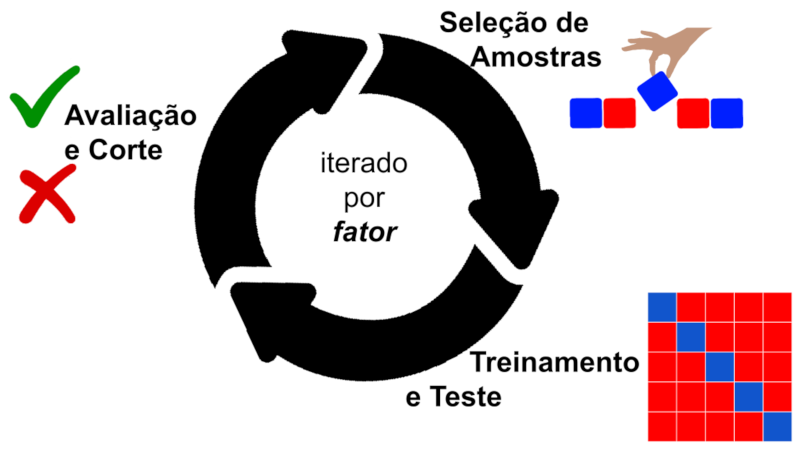
\includegraphics[width=0.5\textwidth]{FIGURES/fig_29.png}
    \caption{Fluxo geral de execução da técnica de avaliação de hiperparâmetros \textit{Halving Random Search with Cross Validation}. Fonte: Elaborada pelo autor.}
    \label{fig:29}
\end{figure}

Uma das formas que a HRSCV possui para limitar o seu custo computacional é definir as condições de parada de sua execução, sendo elas: (a) não haver mais combinações de hiperparâmetros a serem comparados e (b) não haver mais amostras suficientes para iniciar um novo ciclo. A primeira condição, basicamente, indica que foi encontrado o melhor modelo dentro de todas as combinações de hiperparâmetros. Já a segunda condição sinaliza que não há um conjunto de amostras com o tamanho necessário para iniciar o ciclo, sendo finalizada a HRSCV contendo não o vencedor, mas uma lista de N melhores combinações de hiperparâmetros até o momento, em ordem decrescente de pontuação. Conforme já definimos anteriormente, as propostas deste capítulo utilizam como métrica para esta pontuação o valor de \textit{F1-Score}.

Expostas essas informações, é possível estimar quantos ciclos de execução são executados, com base nos valores iniciais da técnica HRSCV, cujos valores de combinações e amostras são, respectivamente, calculados pelas equações \ref{eq:9} e \ref{eq:10}. O tamanho de combinações de hiperparâmetros inicial já é conhecido (9.526.572) e o valor de $fator$ deve ser adequado ao problema, mas obrigatoriamente maior que 1. Vamos manter o tamanho de $fator$ padrão, que é de 2, ou seja, a cada ciclo, o número de combinações cai pela metade enquanto o tamanho da amostra dobra. Por fim, devemos definir a quantidade de amostras que são utilizadas no primeiro ciclo da HRSCV. Em sua documentação em \citet{bib:halvingrandomsearch}, o recomendado é que este valor seja no mínimo cinco vezes $fator$ amostras por número de atributos usados para treinar o modelo. Como veremos na seção \ref{cap:7.4}, são utilizados 25 atributos para treinamento dos modelos; logo, o recomendado é utilizar ao menos 250 amostras no primeiro ciclo.

\begin{equation}
    \label{eq:9}
    Amostras_{ciclo}=Amostras_{inicial}*fator^{ciclo - 1}
\end{equation}

\begin{equation}
    \label{eq:10}
    Combinacoes_{ciclo}=Combinacoes_{inicial}*fator^{ciclo - 1}
\end{equation}

Conhecendo as condições de início da HRSCV aplicadas para geração dos modelos propostos, é possível estimar quantos ciclos seriam executados para cada um dos subconjuntos de treinamento, conforme explicitados na Tabela \ref{tab:XXIV}. Nesta tabela, apresentamos todos os ciclos possíveis até atingir a condição de parada (a), ou seja, de encontrar a melhor combinação de hiperparâmetros. Todavia, não temos um conjunto de treinamento que contenha dois bilhões de amostras, como exigiria o 24$^\circ$ ciclo apresentado na Tabela \ref{tab:XXIV}. Ainda assim, evidenciamos que o menor conjunto de treinamento (profundidade 0 para o CQ 55, conforme Tabela \ref{tab:XXII}), pode ser processado em oito ciclos, retornando uma lista com mais de 37 mil combinações de hiperparâmetros. Já o maior conjunto de treinamento (da profundidade 2 para o CQ 20), pode ser processado em 11 ciclos, retornando uma lista com 9 mil combinações de hiperparâmetros.

\begin{table}
\begin{center}
\caption{Número de candidatos e amostras necessárias para execução de cada ciclo da técnica HRSCV, conforme condições definidas nesta tese.}
\label{tab:XXIV}
\footnotesize

\begin{tblr}{
    colspec = {l|r|r},
    hlines,
    row{even} = {gray9}
}
\hline

\textbf{Ciclo} & \textbf{Candidatos} & \textbf{Amostras}      \\
1     & 9.526.572  & 250           \\
2     & 4.763.286  & 500           \\
3     & 2.381.643  & 1.000         \\
4     & 1.190.822  & 2.000         \\
5     & 595.411    & 4.000         \\
6     & 297.705    & 8.000         \\
7     & 148.853    & 16.000        \\
8     & 74.426     & 32.000        \\
9     & 37.213     & 64.000        \\
10    & 18.607     & 128.000       \\
11    & 9.303      & 256.000       \\
12    & 4.652      & 512.000       \\
13    & 2.326      & 1.024.000     \\
14    & 1.163      & 2.048.000     \\
15    & 581        & 4.096.000     \\
16    & 291        & 8.192.000     \\
17    & 145        & 16.384.000    \\
18    & 73         & 32.768.000    \\
19    & 36         & 65.536.000    \\
20    & 18         & 131.072.000   \\
21    & 9          & 262.144.000   \\
22    & 5          & 524.288.000   \\
23    & 2          & 1.048.576.000 \\
24    & 1          & 2.097.152.000 \\
\hline
\end{tblr}
\end{center}
\end{table}


De cada uma dessas 12 listas retornadas ao fim da execução da HRSCV, capturamos os 20 melhores, unificando-os para obter uma lista de até 240 combinações de hiperparâmetros. há a possibilidade de existirem combinações repetidas nas listas, logo, as repetições são eliminadas. Só então, aplicamos o treinamento e o teste completo para os modelos, de forma a gerar uma lista com dados estatísticos de todos esses candidatos. Com esses processos de filtragem, reduzimos o tempo de processamento de 21 anos de uma busca exaustiva para menos de 10 horas.

Em posse da lista dos 240 candidatos e dos seus valores estatísticos, removemos todos os que não atingem ao menos 0,75 pontos de AUC, mesmo que para apenas um único modelo. Como a AUC informa a probabilidade de o modelo retornar uma resposta positiva corretamente, determinamos que o mínimo valor aceitável seja de 0,75, por ser a metade entre o pior (0,5) e o melhor (1,0) AUC possível. Após essa filtragem final, calculamos a média do \textit{F1-Score} de todos os modelos que foram treinados sob uma mesma combinação de hiperparâmetros, ordenando-os por valor de \textit{F1-Score} médio. Aquele candidato que estiver em primeiro lugar nesta lista, será utilizado na Fase 4 do \textit{pipeline}, a fim de ser aplicado na aceleração da transcodificação.

\section{Transcodificação Rápida para o AV1}
\label{cap:7.4}

Nesta seção, apresentamos as modificações realizadas nos diversos decodificadores e no codificador de referência do AV1 para permitir o desenvolvimento da transcodificação rápida proposta neste capítulo, indicando pontos que são compartilhados em diversas fases de execução do \textit{pipeline} proposto. Para possibilitar uma apresentação mais clara, o conteúdo encontra-se dividido em dois pontos: proposta de algoritmo de transcodificação rápida (subseção \ref{cap:7.4.1}) e modificações necessárias para adequar os decodificadores ao algoritmo desenvolvido de transcodificação rápida (subseção \ref{cap:7.4.2}).

\subsection{Proposta de Algoritmo de Transcodificação Rápida}
\label{cap:7.4.1}

Antes de apresentar a nossa proposta, se faz necessário compreender o fluxo de execução do algoritmo de particionamento de blocos do software de referência do AV1, em sua versão 3.5.0, representado na Figura \ref{fig:30}. Nesta figura, observam-se quatro conjuntos principais de processos: 

\begin{itemize}
    \item \textbf{Blocos verdes}, indicando de início e fim de processos;

    \item \textbf{Blocos cinzas}, indicando processos de predição intraquadro ou interquadros nos blocos daquele tipo de particionamento;

    \item \textbf{Blocos azuis}, indicando processos de podas antecipadas realizadas através de modelos preditivos nativos do \textit{libaom};

    \item \textbf{Bloco branco}, indicando um condicional que avalia se as podas realizadas não geraram situação impossível, por exemplo, uma repetição infinita ou uma impossibilidade de obter melhores resultados de custo taxa-distorção (rd-cost).
\end{itemize}

\begin{figure}
    \centering
    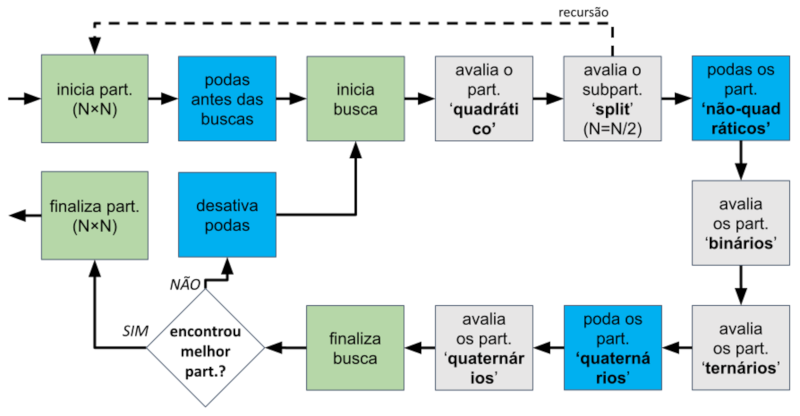
\includegraphics[width=0.75\textwidth]{FIGURES/fig_30.png}
    \caption{Diagrama de execução da busca da melhor estrutura de particionamentos no \textit{libaom} 3.5.0. Fonte: Elaborada pelo autor.}
    \label{fig:30}
\end{figure}

Há uma recursão explícita no fluxo de particionamento de blocos do AV1, conforme pode ser observado na Figura \ref{fig:30}. Recursão essa que é aplicada para quatro novos processos, cada um relacionado a um novo ramo da árvore de particionamentos. Nas versões anteriores do \textit{libaom}, era obrigatório o teste de predição intraquadro ou interquadros no bloco em processamento com ao menos um modo de predição, o que explica a obrigatoriedade da predição simples aplicada ao nosso trabalho de H.265/HEVC-para-AV1 na seção \ref{cap:6.1}. Contudo, na versão atual do \textit{libaom}, é possível ignorar a predição, caso o processo de podas realizado antes das buscas assim identifique. Neste caso, apenas o modo de particionamento \textit{SPLIT} é executado, ou seja, a recursão é aplicada.

Como já foi esclarecido, os modelos preditivos gerados na proposta de transcodificador rápido decidem sobre o particionamento ou não do bloco atual. Logo, modificamos o fluxo de execução do particionamento de blocos da Figura \ref{fig:30} para incluir os processos de antecipação do modo \textit{SPLIT}, realizado através dos modelos preditivos propostos neste capítulo, conforme pode ser visto em laranja na Figura \ref{fig:31}.

\begin{figure}
    \centering
    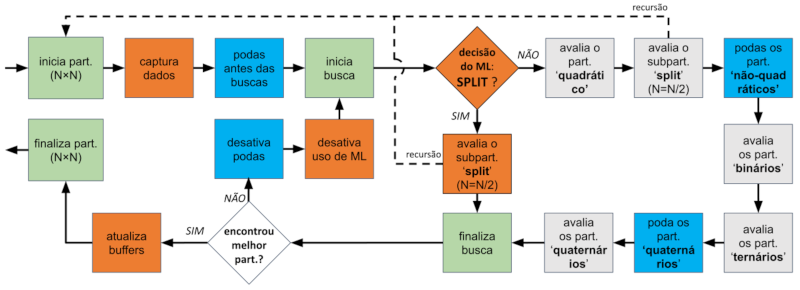
\includegraphics[width=\textwidth]{FIGURES/fig_31.png}
    \caption{Diagrama de execução da busca da melhor estrutura de particionamentos no transcodificador rápido (\textit{libaom} 3.5.0). Fonte: Elaborada pelo autor.}
    \label{fig:31}
\end{figure}

Na Figura \ref{fig:31} observam-se cinco modificações (destacados em laranja), cada uma responsável por um processo específico, conforme descrevemos abaixo:

\begin{enumerate}[1.]
    \item Selecionar informações nos \textit{buffers} que alimentam o modelo preditivo;

    \item Avaliar respostas dos modelos preditivos propostos;

    \item Utilizar o tipo de particionamento \textit{SPLIT}, caso os modelos propostos assim indiquem;

    \item Desativar o modelo de aprendizado de máquina proposto, caso o condicional do fluxo principal de execução do particionamento de blocos do \textit{libaom} assim o indique;

    \item Atualizar informações processadas aos \textit{buffers} que alimentam o modelo preditivo proposto.
\end{enumerate}

Dentre esses cinco processos implementados no fluxo de execução do particionamento de blocos, destacam-se dois: atualização de \textit{buffers} e captura de dados. O primeiro destes processos tem como objetivo ler as informações extraídas tanto do decodificador como do codificador e armazená-las em estruturas de dados que, durante o segundo destes processos, alimentará os modelos preditivos. É após a resposta positiva do condicional do fluxo de execução do particionamento de blocos que se torna possível a obtenção das decisões obtidas naquele nível de profundidade do AV1. Logo, a atualização das estruturas de dados que alimentam o modelo preditivo só ocorre neste momento, independente da profundidade processada. Os tipos de dados extraídos, tanto do decodificador como do codificador, são idênticos, pois dessa forma se reduz significativamente a complexidade de adaptação de estruturas de dados e modificações de tipos de dados ao adaptar o algoritmo de transcodificador rápido para outros formatos. Portanto, as seguintes variáveis são coletadas:

\begin{enumerate}[1.]
    \item \textbf{Nível de Profundidade}: indica quantas vezes a árvore de particionamento se dividiu. Essa variável está diretamente ligada ao rótulo a ser predito. Esperam-se valores inteiros e maiores que 0, onde 0 indica que o superbloco não se subdividiu (ou seja, um bloco quadrático equivalente a 128$\times$128). O valor máximo esperado é 5, onde a árvore atingiu a profundidade máxima, ou seja, bloco de tamanho 4$\times$4. Ressalta-se que atribuímos 0 para blocos 128$\times$128, pois este é o maior tamanho de bloco atualmente disponível nos formatos de codificação de vídeo;

    \item \textbf{Tamanho de bloco}: informa um código referente ao tamanho de bloco utilizado. É relevante utilizar essa variável em conjunto com a anterior porque, apesar de ser possível inferir a profundidade da árvore por meio do tamanho de bloco, o inverso não é verdade. Por exemplo, o bloco 32$\times$32 em essência está na profundidade 2, mas caso o AV1 utilize algum tipo de particionamento ternário (tipo \textit{AB}), esse mesmo tamanho de bloco estará, na verdade, na profundidade 1. São esperados valores inteiros, correspondentes à identificação interna do software do codificador para esses tamanhos de blocos;

    \item \textbf{Orientação dos blocos}: informa qual é a orientação dos blocos não quadráticos utilizados naquela profundidade. Essa variável complementa as duas variáveis anteriores, pois auxilia a identificar o tamanho do bloco com a profundidade. São esperados valores inteiros, onde 0 indica o uso de blocos quadráticos, código 1 indica orientação horizontal e código 2 indica orientação vertical; 

    \item \textbf{Modo de predição}: informa o código do modo de predição intraquadro ou interquadros utilizado pelo codificador;

    \item \textbf{Tipo de predição}: complementa a variável anterior, indicando qual foi o tipo de predição realizado, se intraquadro (código 0) ou interquadros (código 1). Essa variável é utilizada porque há uma tendência de blocos menores serem codificados com predição do tipo intraquadro, o que pode auxiliar o modelo a identificar possíveis subparticionamentos de blocos.
\end{enumerate}

No algoritmo de transcodificação rápido desenvolvido, sumarizado na Figura \ref{fig:31}, as informações que alimentam os modelos preditivos são capturadas e armazenadas em \textit{buffers}, que contêm todas as variáveis acima citadas de regiões vizinhas ao bloco em processamento (B.P.). A escolha por regiões vizinhas como fonte de informações para uso em modelos preditivos já foi observada em \citet{bib:guo_2018}, indicando que é particularmente mais eficiente em vídeos de resolução HD1080 ou superior. Desta forma, representamos na Figura \ref{fig:32} as regiões nas quais as variáveis acima citadas serão capturadas, a fim de alimentar o modelo preditivo. Nesta figura, observam-se cinco regiões (A, B, C, D e E) distantes N pixels da posição do B.P., nas quais serão capturados cinco valores de cada uma. Logo, os modelos preditivos utilizados nas soluções propostas neste capítulo utilizam 25 atributos para embasar as suas decisões. Observe que, por utilizarmos regiões vizinhas ao B.P., as regiões B, C, D e E, eventualmente, podem estar localizadas aquém dos limites do quadro, isto é, suas posições x e y podem ser menores que zero. Nesses casos excepcionais, os modelos preditivos estarão desabilitados para uso naquela iteração da busca da melhor estrutura de particionamentos no \textit{libaom}.

\begin{figure}
    \centering
    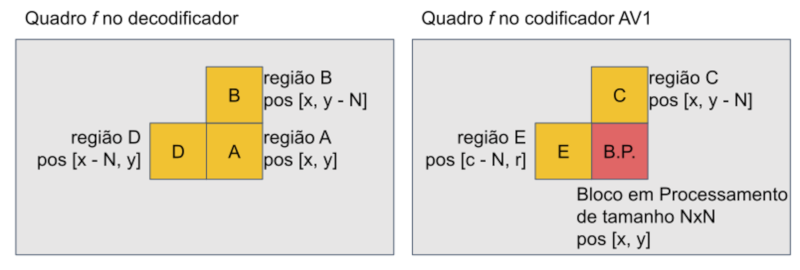
\includegraphics[width=0.75\textwidth]{FIGURES/fig_32.png}
    \caption{Representação em alto nível das regiões onde atributos são selecionados para alimentar o modelo preditivo. Fonte: Elaborada pelo autor.}
    \label{fig:32}
\end{figure}

Sete matrizes compõem as estruturas de dados utilizadas para armazenar as informações, sendo quatro dedicadas ao armazenamento das informações provenientes do decodificador, quatro para armazenar as decisões do codificador e uma matriz auxiliar (AUX) utilizada para preenchimento das seis matrizes anteriores. É nesta matriz AUX que serão armazenadas todas as informações observadas durante a decodificação e a re-codificação, em áreas de 4$\times$4 pixels e, desta forma, utilizadas para alimentar corretamente as outras matrizes. Cada uma das matrizes principais são utilizadas para o armazenamento de informações relativas ao nível de profundidade ao qual estão associadas. Conforme pode ser visto na Figura \ref{fig:33}, cada uma das matrizes principais possui um tamanho distinto e proporcional à resolução do vídeo, onde cada ponto (P) dessa matriz representa uma área de igual tamanho de bloco ao qual está sendo processado (128$\times$128, 64$\times$64 ou 32$\times$32). Assim, considerando um vídeo de resolução HD1080, a matriz com P igual a 128$\times$128 terá o tamanho de 15$\times$9. Ao final do processo ``\textit{Atualiza Buffers}'', apresentado na Figura \ref{fig:32}, a matriz auxiliar é utilizada para geração de médias que preencherão as matrizes principais.

\begin{figure}
    \centering
    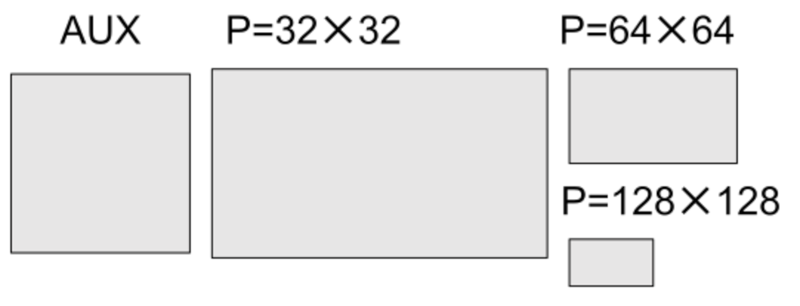
\includegraphics[width=0.5\textwidth]{FIGURES/fig_33.png}
    \caption{Representação do tamanho das matrizes utilizadas pelas estruturas de dados implementadas. Fonte: Elaborada pelo autor.}
    \label{fig:33}
\end{figure}

\subsection{Informações Extraídas dos Softwares Decodificadores}
\label{cap:7.4.2}

Na subseção anterior apresentamos o algoritmo proposto para transcodificação rápida para o formato AV1, cuja estrutura geral pode ser adaptada para demais propostas de transcodificador. Como discutido na subseção anterior, todas as regiões apresentadas na Figura \ref{fig:32} armazenam os mesmos tipos de informações. Logo, cada um dos decodificadores considerados precisam exportar as mesmas informações, na medida que isso seja possível. Nesta subseção, discutimos de que forma isso foi implementado.

Um dos dados exportados não versa sobre nenhuma das cinco variáveis necessárias para preenchimento das matrizes principais, mas identifica a posição do bloco ao qual correspondem as informações no quadro decodificado. Enquanto os padrões H.265/HEVC e H.266/VVC utilizam posições reais de pixels para identificar regiões do quadro, ou seja, um bloco na posição [384, 512] está de fato nesta posição no quadro, no padrão H.264/AVC e nos formatos VP8, VP9 e AV1, cada posição de bloco não é um valor absoluto de pixel, mas um referencial para o menor conjunto de blocos existente naquele formato. Dessa forma, a posição [384, 512] no formato AV1 indica um bloco localizado a partir do pixel [1536, 2048], por exemplo. Portanto, as posições de bloco representadas em cada decodificador precisam ser adequados para o formato utilizado pelo AV1, seguindo as regras abaixo:

\begin{itemize}
    \item Se a posição for originária de um vídeo no formato VP8 ou do padrão H.264/AVC, multiplicar os valores na tupla por quatro;

    \item Se a posição for originária de um vídeo no formato VP9, multiplicar os valores da tupla por dois;

    \item Se a posição for originária de um vídeo codificado nos padrões H.265/HEVC ou H.266/VVC, dividir os valores da tupla por quatro.
\end{itemize}

Já em relação à obtenção das variáveis propriamente ditas, as duas que não precisam ser adaptadas em nenhum dos cinco formatos utilizados na decodificação (VP8, VP9, H.264/AVC, H.265/HEVC e H.266/VVC) são as variáveis ``\textit{Orientação do Bloco}'' e ``\textit{Modo de Predição}''. No caso da primeira, basta observar os tamanhos de blocos utilizados; na segunda, exporta-se a informação sem nenhum de adaptação de valores, já que cada formato de codificação possui uma identificação numérica própria para esses modos de predição. Dessa forma, preferimos manter essa identificação inalterada. A variável ``\textit{Nível de Profundidade}'', como discutido na subseção anterior, contabiliza o número de vezes que o modo \textit{SPLIT} foi escolhido. No entanto, apenas o padrão H.266/VVC possui nível zero, por ser o único formato que oferece tamanho de bloco igual a 128$\times$128, além do AV1. Para todos os demais formatos, adaptou-se a contagem de particionamentos para torná-la equivalente à numeração observada no formato AV1. A única exceção recai para o VP8, que só possui dois tamanhos de blocos: 16$\times$16 e 4$\times$4; logo, há somente dois níveis de profundidades no VP8: 3 e 5.

Ainda no formato VP8, o tamanho de bloco utilizado já indica o tipo de predição realizado, isto é, se intraquadro (blocos 4$\times$4) ou interquadros (blocos 16$\times$16). Por outro lado, apesar dos formatos H.265/HEVC e H.266/VVC compartilharem a variável que indica se o tipo de predição é intraquadro ou interquadros, o tamanho de bloco não é fator decisivo para essa informação. Inclusive, esses dois padrões possuem uma complexa estrutura de particionamentos (como visto no capítulo \ref{cap:2}), havendo uma estrutura composta por sub-estruturas, cada uma com uma finalidade específica para a codificação, vide \citet{bib:h265} e \citet{bib:vvc_partitioningStructure}. Como essas estruturas não são repassadas ao decodificador, não é possível obter diretamente maiores informações sobre elas. No decodificador, podem-se obter apenas informações sobre a largura e a altura dos blocos, o que utilizamos para inferir as variáveis de ``\textit{Tamanho de Bloco}'' e ``\textit{Orientação do Bloco}''.

\section{Resultados}
\label{cap:7.5}

No capítulo \ref{cap:4} descrevemos todas as condições dos experimentos a serem realizados nesta tese e também abordamos o algoritmo desenvolvido para possibilitar uma transcodificação acelerada de VP9 para o AV1, adaptando-se a proposta para diversos formatos, conforme já abordado na seção \ref{cap:7.4}. Logo, seguindo-se a ordem cronológica de publicação dos formatos, conforme visto na Figura \ref{fig:1}, cinco transcodificadores foram implementados utilizando o \textit{pipeline} de processamento proposto: VP9 para AV1 (subseção \ref{cap:7.5.1}), H.264/AVC para AV1 (\ref{cap:7.5.2}), VP8 para AV1 (\ref{cap:7.5.3}), H.265/HEVC para AV1 (\ref{cap:7.5.4}) e H.266/VVC para AV1 (\ref{cap:7.5.5}). 

Antes de apresentar e discutir os resultados de transcodificação, vale destacar quais foram os modelos candidatos vencedores de cada uma das propostas implementadas, ou seja, a combinação de hiperparâmetros aprovados na Fase 3 do \textit{pipeline} (como visto na subseção \ref{cap:7.2.3} e seção \ref{cap:7.3}). A Tabela \ref{tab:XXV} apresenta a configuração de hiperparâmetros para cada um dos transcodificadores propostos neste capítulo. É possível observar que os quatro hiperparâmetros foram os mesmos em todos os treinamentos realizados na Fase 3: \textit{criterion} como ``\textit{entropy}'', \textit{splitter} como ``\textit{best}'', \textit{max depth} como 11 e \textit{min impurity decrease} como 0,60. Ou seja, em qualquer modelo preditivo treinado nas condições que impusemos, até 11 níveis de profundidade da árvore de decisão são permitidos, onde cada subparticionamento dessa árvore é feita pela melhor escolha possível, considerando uma impureza mínima de 0,60 pontos e utilizando o ganho de informação de Shannon que, segundo \citet{bib:CART_matematica} e \citet{bib:shannon_entropy}, quantifica a desordem dos dados em comparação com uma variável aleatória constante. Em outras palavras, o ganho de informação de Shannon identifica a desigualdade da informação e auxilia na tomada de decisão sobre qual atributo deve ser utilizado no particionamento da árvore de decisão. 

\begin{table}
\begin{center}
\caption{Configuração dos candidatos vencedores a serem usados nas transcodificações aceleradas para o formato AV1.}
\label{tab:XXV}
\footnotesize

\begin{tblr}{
    colspec = {c|c|c|c|c|c},
    hlines,
    row{even} = {gray9}
}
\hline
\textbf{Hiperparâmetro} & \textbf{VP9} & \textbf{H.264/AVC} & \textbf{VP8} & \textbf{H.265/HEVC} & \textbf{H.266/VVC}\\
Criterion & entropy & entropy & entropy & entropy & entropy\\
Splitter & best & best & best & best & best\\
Max Depth & 11 & 11 & 11 & 11 & 11\\
Min Samples Split & 11 & 17 & 17 & 17 & 11\\
Min Samples Leaf & 11 & 13 & 13 & 13 & 11\\
Max Features & sqrt & None & None & None & sqrt\\
Max Leaf Nodes & 7 & 19 & 19 & 19 & 7\\
Min Impurity Decrease & 0,6 & 0,6 & 0,6 & 0,6 & 0,6\\
CPP Alpha & 0,5 & 0,4 & 0,4 & 0,4 & 0,5\\
\hline
\end{tblr}
\end{center}
\end{table}


Além dos quatro hiperparâmetros que são fixos nas cinco propostas de transcodificação rápida, observamos que os demais hiperparâmetros compõem dois conjuntos de configurações, que podem ser resumidos pelo \textit{max leaf nodes}, ou seja, a quantidade máxima de nós-folha da árvore de decisão, se 7 (transcodificadores VP9 e H.266/VVC) ou 19 (transcodificadores H.264/AVC, VP8 e H.265/HEVC). A proximidade dos valores dos hiperparâmetros, mesmo sob transcodificadores distintos, se explica pois os 25 atributos utilizados nas cinco propostas são os mesmos (médias de algum valor), inclusive havendo dez desses atributos tendo origem do mesmo codificador AV1. Apesar disso, os valores presentes nesses atributos podem variar e, consequentemente, as árvores geradas também serão diferentes. Como exemplo, apresentamos a Figura \ref{fig:34}, que mostra um modelo gerado para o formato VP9, para a profundidade 2 e CQ 43. Como é possível ver nesta figura, apesar da profundidade máxima ser 11, o modelo optou por ir até a profundidade 7. Também é possível observar a utilização de somente alguns atributos dos 25 disponíveis e, neste modelo preditivo em especial, foram utilizados os atributos de média de profundidade da zona A (decodificador, mesma posição do bloco em processamento); do tamanho do bloco da zona A; do tamanho do bloco da zona B (decodificador, posição acima do bloco em processamento); da orientação do bloco na zona B; da profundidade da zona C (codificador, posição acima do bloco em processamento); e do modo de predição da zona C.

\begin{figure}
    \centering
    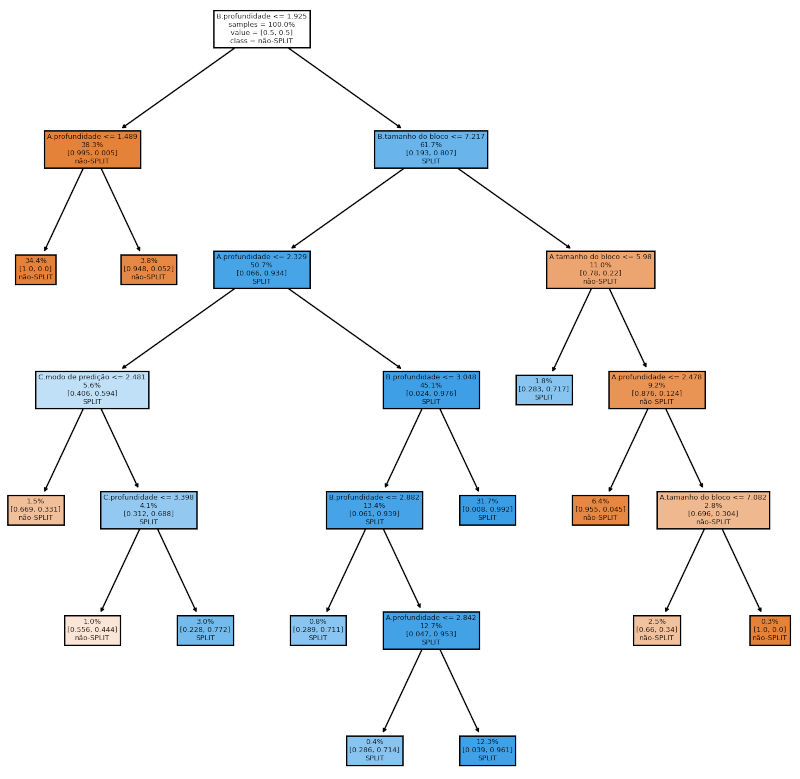
\includegraphics[width=\textwidth]{FIGURES/fig_34.png}
    \caption{Uma árvore de decisão gerada pelos modelos propostos. Fonte: Elaborada pelo autor.}
    \label{fig:34}
\end{figure}

Destes 12 modelos treinados com o conjunto completo de dados de treinamento, conforme explicitado na subseção \ref{cap:7.2.3}, e configurados conforme a Tabela \ref{tab:XXV}, foi possível obter os valores de F1-Score para todos os modelos e todas as propostas de transcodificador, conforme apresentados na Tabela \ref{tab:XXVI}. Nesta tabela, evidenciamos que a média obtida para a transcodificação de VP9 para AV1 é a maior de todas, apesar de que todas as demais apresentam valores muito próximos. Portanto, a expectativa é que os resultados de transcodificação sejam também próximos, principalmente relacionados ao impacto na eficiência da codificação. Analisando os resultados individuais de cada modelo presente na Tabela \ref{tab:XXVI}, é possível notar que o valor de \textit{F1-Score} decai conforme a profundidade aumenta. Por exemplo, o modelo do CQ 20 e profundidade 0 do transcodificador de H.266/VVC para AV1 possui um \textit{F1-Score} de 0,9929, enquanto que o modelo relacionado à profundidade 2 possui o valor de 0,9412. Apesar de ser uma diferença pequena, que se reflete em maior ou menor grau nos demais casos similares, hipotetiza-se que essa diferença implique em um erro de decisão maior nas sequências que requisitem uma profundidade maior da árvore de particionamento. Em outras palavras, vídeos que necessitem de maiores detalhes devem ter um impacto na eficiência de codificação maior que em sequências onde blocos grandes são mais utilizados, basicamente, em cenas mais paradas ou com grandes áreas homogêneas. 

\begin{table}
\begin{center}
\caption{Resultados da métrica \textit{F1-Score} obtidos com os modelos preditivos treinados sob os candidatos vencedores de cada proposta de transcodificação acelerado implementado.}
\label{tab:XXVI}
\footnotesize

\begin{tblr}{
    colspec = {l|r|r|r|r|r},
    hlines,
    row{even} = {gray9}
}
\hline
\textbf{Modelo do Conjunto} & \textbf{VP9} & \textbf{H.264/AVC} & \textbf{VP8} & \textbf{H.265/HEVC} & \textbf{H.266/VVC}\\
1 (CQ 20 P 0) & 0,9919 & 0,9917 & 0,9926 & 0,9928 & 0,9929\\
2 (CQ 20 P 1) & 0,9552 & 0,9796 & 0,9774 & 0,9551 & 0,9588\\
3 (CQ 20 P 2) & 0,9592 & 0,9362 & 0,9480 & 0,9480 & 0,9412\\
4 (CQ 32 P 0) & 0,9933 & 0,9928 & 0,9929 & 0,9933 & 0,9932\\
5 (CQ 32 P 1) & 0,9608 & 0,9560 & 0,9513 & 0,9554 & 0,9507\\
6 (CQ 32 P 2) & 0,9508 & 0,9535 & 0,9450 & 0,9520 & 0,9448\\
7 (CQ 43 P 0) & 0,9932 & 0,9931 & 0,9939 & 0,9930 & 0,9934\\
8 (CQ 43 P 1) & 0,9500 & 0,9447 & 0,9484 & 0,9520 & 0,9494\\
9 (CQ 43 P 2) & 0,9445 & 0,9418 & 0,9393 & 0,9419 & 0,9465\\
10 (CQ 55 P 0) & 0,9934 & 0,9935 & 0,9933 & 0,9934 & 0,9933\\
11(CQ 55 P 1) & 0,9591 & 0,9512 & 0,9552 & 0,9571 & 0,9465\\
12 (CQ 55 P 2) & 0,9330 & 0,9398 & 0,9344 & 0,9324 & 0,9389\\
\textbf{Média} & \textbf{0,9654} & \textbf{0,9645} & \textbf{0,9643} & \textbf{0,9639} & \textbf{0,9625}\\
\hline
\end{tblr}
\end{center}
\end{table}


Por fim, antes de apresentar os resultados obtidos, é preciso relembrar que a média de aceleração observada na literatura, conforme foi visto no capítulo \ref{cap:3}, é de 50,74\% de TS e de 4,11\% de BD-rate. Também ressaltamos neste capítulo que a comparação direta de qualquer solução com a média observada não pode ser feita de forma justa, haja visto a necessidade de se equiparar não apenas os formatos de transcodificação, como também as sequências utilizadas, as configurações aplicadas e a aplicabilidade alvo da proposta. Destacado essa injustiça ao se realizar qualquer comparação, nesta tese serão aplicadas comparações superficiais com a média, tendo em vista a ausência de melhores trabalhos para comparações. Ressalta-se, ainda, que mesmo propostas com valores com menor destaque ao observado na média da literatura não implicam diretamente em propostas ruins, pois, como já dissemos, quaisquer análises de resultados desconsideram contextos intrínsecos dos trabalhos desenvolvidos naquelas propostas, tampouco sobre os formatos de transcodificação utilizados. Dessa forma, apesar do uso de correlações com a média observada na literatura ter seu propósito de criar expectativas, essa análise não valida ou invalida quaisquer resultados.


\subsection{Transcodificação Rápida de VP9-para-AV1}
\label{cap:7.5.1}

A Tabela \ref{tab:XXVII} dispõe de todos os resultados obtidos para o transcodificador rápido de VP9 para AV1. Observa-se uma aceleração média da transcodificação de 16,76\%, a um custo de elevar o BD-rate em 5,10\%. Os três melhores resultados desta transcodificação estão na resolução HD1080, cuja resolução foi utilizado para realizar os treinamentos dos modelos preditivos. Nesta resolução em especial (HD1080), observa-se um TS de 19,58\% e um BD-rate de 4,47\%. As três sequências que apresentaram maior destaque são: \textit{crowd\_run\_1080p50\_60f}, \textit{ducks\_take\_off\_1080p50\_60f} e \textit{guitar\_hdr\_amazon\_1080p}, respectivamente com acelerações iguais a 36,81\%, 37,35\% e 51,96\%. Inclusive, a sequência \textit{guitar\_hdr\_amazon\_1080p} apresentou o maior TS entre todos os resultados de transcodificação rápida de VP9 para AV1. Apesar de serem sequências com cenas bem distintas (como pode ser visto no Apêndice \ref{apx:A}), indo desde patos nadando em um lago até um grupo de pessoas correndo montanha abaixo, há algo que é similar entre eles: são cenas de movimento em toda a área do quadro. Isso indica que as sequências devam usar uma quantidade maior de blocos menores, sugerindo que os modelos preditivos, pelo menos para as profundidades 0 e 1, são eficientes em predizer corretamente o particionamento do bloco.

\begin{center}
{\footnotesize
\begin{longtblr}[
    caption = {Resultados da transcodificação rápida de VP9 para AV1 baseado em modelos preditivos.},
    label = {tab:XXVII}
]{
    colspec = {l|p{6cm}|r|r|r},
    hlines,
    row{even} = {gray9}
}
\hline
\textbf{Resolução} & \textbf{Sequência} & \textbf{BD-rate (\%)} & \textbf{TS (\%)} & \textbf{Razão}\\
\SetCell[r=12]{l}HD720 & boat\_hdr\_amazon\_720p & 4,2537 & 13,99 & 0,304\\
 & dark720p\_120f & 5,4006 & 19,44 & 0,278\\
 & FourPeople\_1280x720\_60 & 2,4022 & 7,98 & 0,301\\
 & FourPeople\_1280x720\_60\_120f & 2,3122 & 8,05 & 0,287\\
 & gipsrestat720p\_120f & 2,6988 & 11,76 & 0,229\\
 & Johnny\_1280x720\_60 & 4,0714 & 14,33 & 0,284\\
 & Johnny\_1280x720\_60\_120f & 3,8174 & 15,76 & 0,242\\
 & KristenAndSara\_1280x720\_60 & 3,0265 & 16,69 & 0,181\\
 & KristenAndSara\_1280x720\_60\_120f & 3,0265 & 16,63 & 0,182\\
 & Netflix\_DinnerScene\_1280x720\_60fps \_8bit\_420\_120f & 6,3817 & 27,47 & 0,232\\
 & Netflix\_DrivingPOV\_1280x720\_60fps \_8bit\_420\_120f & 3,0173 & 12,54 & 0,241\\
 & Netflix\_FoodMarket2\_1280x720\_60fps \_8bit\_420\_120f & 2,966 & 8,99 & 0,330\\
\SetCell[r=8]{l}HD720 & Netflix\_RollerCoaster\_1280x720\_60fps \_8bit\_420\_120f & 5,7515 & 25,11 & 0,229\\
 & Netflix\_Tango\_1280x720\_60fps\_8bit \_420\_120f & 4,3562 & 8,07 & 0,540\\
 & rain\_hdr\_amazon\_720p & 1,0663 & 7,37 & 0,145\\
 & vidyo1\_720p\_60fps\_120f & 3,2613 & 12,9 & 0,253\\
 & Vidyo3\_1280x720\_60 & 3,8858 & 14,11 & 0,275\\
 & vidyo3\_720p\_60fps\_120f & 3,6996 & 14,16 & 0,261\\
 & Vidyo4\_1280x720\_60 & 2,9377 & 13,09 & 0,225\\
 & vidyo4\_720p\_60fps\_120f & 3,1043 & 12,99 & 0,239\\
\SetCell[c=2]{r}\textbf{Média dos vídeos HD720} && \textbf{3,5718} & \textbf{14,07} & \\
\SetCell[r=17]{l}HD1080 & aspen\_1080p\_60f & 5,7618 & 9,11 & 0,632\\
 & crowd\_run\_1080p50\_60f & 2,736 & 36,81 & 0,074\\
 & ducks\_take\_off\_1080p50\_60f & 4,4386 & 37,35 & 0,119\\
 & guitar\_hdr\_amazon\_1080p & 6,3438 & 51,96 & 0,122\\
 & Netflix\_Aerial\_1920x1080\_60fps\_8bit \_420\_60f & 4,2699 & 29,04 & 0,147\\
 & Netflix\_Boat\_1920x1080\_60fps\_8bit \_420\_60f & 1,7737 & 18,42 & 0,096\\
 & Netflix\_Crosswalk\_1920x1080\_60fps \_8bit\_420\_60f & 3,7432 & 24,88 & 0,150\\
 & Netflix\_FoodMarket\_1920x1080\_60fps \_8bit\_420\_60f & 4,862 & 12,47 & 0,390\\
 & Netflix\_PierSeaside\_1920x1080\_60fps \_8bit\_420\_60f & 3,9322 & 9,41 & 0,418\\
 & Netflix\_SquareAndTimelapse\_1920x 1080\_60fps\_8bit\_420\_60f & 3,7862 & 8,64 & 0,438\\
 & Netflix\_TunnelFlag\_1920x1080\_60fps \_8bit\_420\_60f & 7,6284 & 28,33 & 0,269\\
 & old\_town\_cross\_1080p50\_60f & 7,6534 & 16,34 & 0,468\\
 & park\_joy\_1080p50\_60f & 2,012 & 9,3 & 0,216\\
 & pedestrian\_area\_1080p25\_60f & 4,2314 & 9,42 & 0,449\\
 & rush\_field\_cuts\_1080p\_60f & 2,4349 & 14,08 & 0,173\\
 & rush\_hour\_1080p25\_60f & 4,5744 & 11,41 & 0,401\\
 & seaplane\_hdr\_amazon\_1080p & 3,1675 & 14,68 & 0,216\\
HD1080 & station2\_1080p25\_60f & 7,2066 & 10,69 & 0,674\\
\SetCell[c=2]{r}\textbf{Média dos vídeos HD1080} && \textbf{4,4753} & \textbf{19,58} & \\
\SetCell[r=6]{l}UHD4K & Netflix\_BoxingPractice\_4096x2160 \_60fps\_10bit\_420\_60f & 11,0334 & 18,01 & 0,613\\
 & Netflix\_Dancers\_4096x2160\_60fps \_10bit\_420\_60f & 24,0996 & 17,77 & 1,356\\
 & Netflix\_Narrator\_4096x2160\_60fps \_10bit\_420\_60f & 12,2722 & 22,98 & 0,534 \\
 & Netflix\_RitualDance\_4096x2160\_60fps \_10bit\_420\_60f & 14,1521 & 20,86 & 0,679 &  & \\
 & Netflix\_ToddlerFountain\_4096x2160 \_60fps\_10bit\_420\_60f & 2.8256 & 19,93 & 0,142 \\
 & Netflix\_WindAndNature\_4096x2160 \_60fps\_10bit\_420\_60f & 8,0698 & 3,96 & 2,038
 \\
\SetCell[c=2]{r}\textbf{Média dos vídeos UHD4K} && \textbf{12,0755} & \textbf{17,25}  & \\
\SetCell[c=2]{r}\textbf{Média Geral} && \textbf{5,1010} & \textbf{16,76} & \\
\SetCell[c=2]{r}\textbf{Desvio Padrão Geral} && \textbf{3,9862} & \textbf{9,30} & \\
\hline
\end{longtblr}
}
\end{center}



Se os resultados observados na resolução HD1080 apresentam resultados positivos em algumas condições, adaptar a proposta para uma resolução menor, como HD720, não trouxe impactos negativos. Inclusive, apresenta resultados similares de redução do tempo (média de 14,07\%) e de impacto na eficiência de codificação (média de 3,57\%) em relação aos resultados observados na resolução HD1080. Nesta resolução, a sequência com a menor Razão foi \textit{rain\_hdr\_amazon\_720p}, com 0,145 pontos, originários de uma aceleração de 7,37\% da transcodificação e um BD-rate de 1,06\%. A sequência HD720 que obteve o maior TS foi \textit{Netflix\_DinnerScene\_1280x720\_60fps\_8bit\_420\_120f} com 27,47\%, mas o BD-rate foi de 6,38\%. Coincidentemente, é com esta sequência de vídeo que se observa o maior BD-rate para a resolução HD720. Todavia, quase todos os vídeos UHD4K não apresentaram resultados satisfatórios de eficiência de codificação, com resultados de BD-rate superiores a 8\% e uma aceleração inferior à 22,98\% (vista na sequência \textit{Netflix\_Narrator\_4096x2160\_60fps\_10bit\_420\_60f}). A única exceção é \textit{Netflix\_ToddlerFountain\_4096x2160\_60fps\_10bit\_420\_60f}, que apresenta 2,82\% de BD-rate e 19,93\% de TS. 

Há, publicado na literatura científica, outra proposta de transcodificador rápido de VP9 para AV1, que desenvolvemos e apresentamos na seção \ref{cap:6.2}. Essa proposta apresentou uma redução de complexidade de 28,16\% a um custo na eficiência de codificação de 4,34\%. Essa proposta de transcodificador rápido não utiliza modelos preditivos para auxiliar nas decisões rápidas e, portanto, consegue apresentar uma média geral melhor que a proposta apresentada nesta subseção, baseada em modelos preditivos. Contudo, o trabalho descrito na seção \ref{cap:6.2} utiliza um conjunto menor de vídeos para avaliar os resultados, apesar de apresentar uma maior variedade de resoluções. Se considerarmos apenas as mesmas sequências utilizadas nas duas propostas, obteremos os dados apresentados na Tabela \ref{tab:XXVIII}, onde comparamos diretamente as duas propostas apresentadas nesta tese para a transcodificação rápida de VP9 para AV1.

\begin{table}
\begin{center}
\caption{Relação direta entre as propostas de transcodificador rápido do formato VP9 para o AV1.}
\label{tab:XXVIII}
\footnotesize

\begin{tblr}{
    colspec = {p{4cm}|r|r|r|r|r|r},
    hlines,
    row{even} = {gray9}
}
\hline
& \SetCell[c=3]{c}\textbf{Proposta com Modelos Preditivos} &&& \SetCell[c=3]{c}\textbf{Proposta com Heurística} &&\\
\textbf{Sequência} & \textbf{BD-rate (\%)} & \textbf{TS (\%)} & \textbf{Razão} & \textbf{BD-rate (\%)} & \textbf{TS (\%)} & \textbf{Razão} \\
dark720p\_120f & 5,40 & 19,44 & 0,28 & 4,14 & 23,02 & 0,18 \\
Johnny\_1280x720\_60\_ 120f & 3,82 & 15,76 & 0,24 & 6,05 & 24,74 & 0,24 \\
Netflix\_DrivingPOV\_1280x 720\_60fps\_8bit\_420\_120f & 3,02 & 12,54 & 0,24 & 6,37 & 31,58 & 0,20 \\
Netflix\_RollerCoaster\_ 1280x720\_60fps\_8bit\_420\_120f & 5,75 & 25,11 & 0,23 & 6,69 & 41,73 & 0,16 \\
\SetCell[c=1]{r}\textbf{Média da resolução HD720} & \textbf{4,50} & \textbf{18,21} & \textbf{0,25} & \textbf{5,81} & \textbf{30,27} & \textbf{0,19} \\
crowd\_run\_1080p50\_60f & 2,74 & 36,81 & 0,07 & 3,53 & 34,25 & 0,10 \\
Netflix\_Crosswalk\_1920x 1080\_60fps\_8bit\_420\_60f & 3,74 & 24,88 & 0,15 & 4,00 & 18,01 & 0,22 \\
park\_joy\_1080p50\_60f & 2,01 & 9,30 & 0,22 & 5,86 & 42,67 & 0,14 \\
seaplane\_hdr\_amazon\_ 1080p & 3,17 & 14,68 & 0,22 & 4,98 & 24,53 & 0,20 \\
\SetCell[c=1]{r}\textbf{Média da resolução HD1080} & \textbf{2,91} & \textbf{21,42} & \textbf{0,14} & \textbf{4,60} & \textbf{29,87} & \textbf{0,15} \\
\SetCell[c=1]{r}\textbf{Média Geral} & \textbf{3,71} & \textbf{19,81} & \textbf{0,19} & \textbf{5,20} & \textbf{30,07} & \textbf{0,17}\\
\hline
\end{tblr}
\end{center}
\end{table}


Na Tabela \ref{tab:XXVIII} podemos observar que o impacto na eficiência de codificação gerado pela proposta baseada em modelos preditivos é menor que o da proposta baseada em heurística. Isso significa que os modelos treinados geram decisões mais assertivas, principalmente na resolução HD1080 (2,91\% contra os 4,60\%). Observe que as sequências \textit{crowd\_run\_1080p50\_60f} e \textit{Netflix\_Crosswalk\_1920x1080\_60fps\_8bit\_420\_60f} apresentaram resultados melhores, tanto em BD-rate como em TS, ao utilizar a proposta baseada em modelos preditivos. Todavia, a aceleração geral obtida com as propostas usando modelos preditivos é menor, em especial para a sequência \textit{park\_joy\_1080p50\_60f}, que foi acelerada em 42,67\% na proposta da seção 6.2 contra os 9,30\% da proposta deste capítulo.

Desta forma, foi preciso investigar a causa do valor de TS inferior. Identificou-se que o algoritmo de transcodificação rápida proposto, em especial na manipulação das matrizes citadas na subseção \ref{cap:7.4.1}, consomem um tempo de processamento significativamente elevado no transcodificador. Avaliando a sequência de vídeo \textit{crowd\_run\_1080p50\_60f} sob o nível de quantização 20, na transcodificação original esta tarefa foi executada em 60.466 segundos (ou 16,8 horas), enquanto que na transcodificação rápida a mesma sequência de vídeo foi processada em 42.181 segundos (11,7 horas). Apesar de podermos perceber uma redução do custo computacional em 30\% nesta única sequência, observaram-se 2.974 segundos (49,6 minutos) do tempo do transcodificador dedicados ao algoritmo desenvolvido, isto é, 7,05\%. O mesmo se observou em outra sequência de vídeo (\textit{pan\_hdr\_amazon\_1080p}) sob um nível de quantização diferente (CQ 43), que codificou em 24.484 segundos na transcodificação original contra os 19.424 segundos na transcodificação rápida, ou seja, atingiu uma redução de 20\% do tempo. No entanto, foram necessários 1.344 segundos na execução do algoritmo, ou seja, 6.92\% do tempo total da codificação do \textit{libaom}. Casos similares puderam ser vistos em outras sequências sob níveis de quantização diferentes, com consumos de tempo próximos a 7\%.

Portanto, conclui-se que é possível obter resultados melhores de redução de tempo, caso o algoritmo desenvolvido seja otimizado, a um teto de 7\%, caso sua execução atinja o tempo real. Assim sendo, dos resultados médios de aceleração da resolução HD1080, apresentados na Tabela \ref{tab:XXVII} (de 19,58\%), seria possível estimar um resultado de TS máximo de 26,57\%.

\subsection{Transcodificação Rápida de H.264/AVC-para-AV1}
\label{cap:7.5.2}

A proposta de transcodificador rápido desenvolvida de VP9 para AV1 foi adaptada de H.264/AVC para AV1, utilizando o \textit{pipeline} de processamento. Utilizando as mesmas sequências de vídeo descritas anteriormente, exceto para vídeos UHD4K, foi possível obter uma aceleração da transcodificação de 25,05\% a um custo de reduzir a eficiência de codificação em 5,58\%, como é possível notar na Tabela \ref{tab:XXIX}. Uma observação geral que pode ser vista nesta proposta de transcodificador, em relação ao caso VP9 para AV1, é que os resultados foram melhores para a resolução HD720, ao invés da resolução HD1080. O TS médio obtido na resolução HD720 foi de 30,52\%, contra os 18,67\% da resolução HD1080. Inclusive, o impacto na eficiência de codificação também é menor na resolução HD720 (5,30\% contra 5,91\%). Como o formato H.264/AVC foi desenvolvido para lidar principalmente com resoluções HD720 ou inferiores, supõe-se que as demais informações dos atributos, além das médias de profundidades e de tamanho de bloco, possam contribuir mais para a tomada de decisão nessas resoluções, mesmo utilizando um modelo preditivo treinado para uma resolução maior.

\begin{center}
{\footnotesize
\begin{longtblr}[
 caption = {Resultados da transcodificação rápida de H.264/AVC para AV1 baseada em modelos preditivos.},
 label = {tab:XXIX}
]{
 colspec = {l|p{6cm}|r|r|r},
 hlines,
 row{even} = {gray9}
}
\hline
\textbf{Resolução} & \textbf{Sequência} & \textbf{BD-rate (\%)} & \textbf{TS (\%)} & \textbf{Razão}\\
\SetCell[r=21]{c}HD720 & boat\_hdr\_amazon\_720p & 0,7029 & 12,91 & 0,054 \\
 & dark720p\_120f & 9,1593 & 42,26 & 0,217 \\
 & FourPeople\_1280x720\_60 & 2,6325 & 32,32 & 0,081 \\
 & FourPeople\_1280x720\_60\_120f & 2,5755 & 32,47 & 0,079 \\
 & gipsrestat720p\_120f & 3,6448 & 40,85 & 0,089 \\
 & Johnny\_1280x720\_60 & 7,7357 & 48,34 & 0,160 \\
 & Johnny\_1280x720\_60\_120f & 8,0233 & 49,13 & 0,163 \\
 & KristenAndSara\_1280x720\_60 & 6,0619 & 47,96 & 0,126 \\
 & KristenAndSara\_1280x720\_60\_120f & 6,0619 & 47,97 & 0,126 \\
 & Netflix\_DinnerScene\_1280x720\_60fps \_8bit\_420\_120f & 13,0913 & 37,94 & 0,345 \\
 & Netflix\_DrivingPOV\_1280x720\_60fps \_8bit\_420\_120f & 4,3667 & 17,2 & 0,254 \\
 & Netflix\_FoodMarket2\_1280x720\_60fps \_8bit\_420\_120f & 4,0778 & 20,33 & 0,201 \\
 & Netflix\_RollerCoaster\_1280x720\_60fps \_8bit\_420\_120f & 6,7889 & 43,18 & 0,157 \\
 & Netflix\_Tango\_1280x720\_60fps\_8bit \_420\_120f & 4,3732 & 9,2 & 0,475 \\
 & rain\_hdr\_amazon\_720p & 0,5833 & 10,98 & 0,053 \\
 & Vidyo1\_1280x720\_60 & 4,1503 & 16,69 & 0,249 \\
 & vidyo1\_720p\_60fps\_120f & 3,9878 & 17,05 & 0,234 \\
 & Vidyo3\_1280x720\_60 & 2,8683 & 8,04 & 0,357 \\
 & vidyo3\_720p\_60fps\_120f & 2,3452 & 8,75 & 0,268 \\
 & Vidyo4\_1280x720\_60 & 9,1446 & 48,11 & 0,190 \\
 & vidyo4\_720p\_60fps\_120f & 8,9525 & 49,16 & 0,182 \\
\SetCell[c=2]{r}\textbf{Média dos vídeos HD720} && \textbf{5,3013} & \textbf{30,52} & \\
\SetCell[r=5]{c}HD1080 & aspen\_1080p\_60f & 15,1526 & 33,99 & 0,446 \\
 & crowd\_run\_1080p50\_60f & 0,8863 & 15,65 & 0,057 \\
 & ducks\_take\_off\_1080p50\_60f & 3,3596 & 25,83 & 0,130 \\
 & guitar\_hdr\_amazon\_1080p & 1,1848 & 12,73 & 0,095 \\
 & Netflix\_Aerial\_1920x1080\_60fps\_8bit \_420\_60f & 5,1584 & 20,96 & 0,246 \\
\SetCell[r=13]{c}HD1080 & Netflix\_Boat\_1920x1080\_60fps\_8bit \_420\_60f & 1,8815 & 20,37 & 0,092 \\
 & Netflix\_Crosswalk\_1920x1080\_60fps \_8bit\_420\_60f & 10,3418 & 12,52 & 0,826 \\
 & Netflix\_FoodMarket\_1920x1080\_60fps \_8bit\_420\_60f & 9,5122 & 19,58 & 0,486 \\
 & Netflix\_PierSeaside\_1920x1080\_60fps \_8bit\_420\_60f & 11,0504 & 41,32 & 0,267 \\
 & Netflix\_SquareAndTimelapse\_1920x 1080\_60fps\_8bit\_420\_60f & 3,0506 & 12,59 & 0,240 \\
 & Netflix\_TunnelFlag\_1920x1080\_60fps \_8bit\_420\_60f & 6,7701 & 17,9 & 0,380 \\
 & old\_town\_cross\_1080p50\_60f & 6,3312 & 21,54 & 0,294 \\
 & park\_joy\_1080p50\_60f & 1,0161 & 12,37 & 0,082 \\
 & pedestrian\_area\_1080p25\_60f & 8,176 & 14,23 & 0,575 \\
 & rush\_field\_cuts\_1080p\_60f & 1,0555 & 13,72 & 0,077 \\
 & rush\_hour\_1080p25\_60f & 8,4783 & 14,01 & 0,605 \\
 & seaplane\_hdr\_amazon\_1080p & 0,324 & 5,71 & 0,057 \\
 & station2\_1080p25\_60f & 12,7702 & 21,11 & 0,605 \\
\SetCell[c=2]{r}\textbf{Média dos vídeos HD1080} && \textbf{5,9166} & \textbf{18,67} & \\
\SetCell[c=2]{r}\textbf{Média Geral} && \textbf{5,5853} & \textbf{25,05} & \\
\SetCell[c=2]{r}\textbf{Desvio Padrão Geral} && \textbf{3,8649} & \textbf{14,28} & \\
\hline
\end{longtblr}
}
\end{center}



Os principais destaques na transcodificação de H.264/AVC para AV1 são para as sequências \textit{boat\_hdr\_amazon\_720p}, \textit{rain\_hdr\_amazon\_720p}, \textit{crowd\_run\_1080p50\_60f} e \textit{seaplane\_hdr\_amazon\_1080p}, todos com menos de 0,06 pontos de Razão. Uma característica entre essas sequências é que há uma metade da cena relativamente estática e outra com muitos movimentos, geralmente de água ou de pessoas distantes. Isso significa que há uma mescla homogênea entre tamanhos de bloco, o que, somado às demais informações extraídas dos atributos do H.264/AVC em relação ao VP9, pode impulsionar uma melhora significativa dos resultados observados nesta proposta de transcodificador rápido.

No entanto, há sete sequências HD1080 na Tabela \ref{tab:XXIX} que podem ser enquadradas como resultados negativos, sendo que quatro delas ultrapassam a marca de 10\% de BD-rate. Em especial \textit{Netflix\_Crosswalk\_1920x1080\_60fps\_8bit\_420\_60f}, que apresenta a maior Razão entre todas as sequências, com 12,52\% de TS e 10,34\% de BD-rate. Nota-se uma inversão completa em relação à proposta de VP9 para AV1, onde esta mesma sequência foi uma das de maior destaque, apresentando 24,88\% de TS e 3,74\% de BD-rate. Não identificamos uma causa para essa inversão específica.

Como visto na Tabela \ref{tab:III}, não há outros trabalhos de transcodificação de H.264/AVC para AV1. Portanto, esta é uma proposta inédita de transcodificador rápido e não existem comparações diretas que possam ser feitas. Todavia, observa-se uma média de aceleração dos trabalhos apresentados na literatura científica com o dobro do percentual apresentado do transcodificador apresentado neste subseção. Apesar de não ser possível fazer uma comparação justa dos resultados deste transcodificador rápido com a média da literatura, como já abordamos no Capítulo \ref{cap:3}, ainda assim a redução média de um quarto do tempo do transcodificador rápido, em relação ao transcodificador original, é um resultado positivo.

Considerando os valores de razão próximos ao apresentado pela proposta desenvolvida nesta subseção (de 0,13), os nossos resultados podem ser comparados diretamente com os valores obtidos por \citet{bib:peixoto_2012} (52,75\% de TS e 5,49\% de BD-rate), \citet{bib:peixoto2_2014} (74,54\% de TS e 8,41\% de BD-rate) e \citet{bib:franche_2017} (87,32\% de TS e 3,28\% de BD-rate). Destes trabalhos, \citet{bib:franche_2017} também utiliza informações provenientes tanto do decodificador como do codificador, apesar de sua proposta ser baseada em heurísticas. Por outro lado, \citet{bib:peixoto2_2014} propõe uma solução baseada em modelos preditivos gerados por \textit{Linear Discriminant Function} \cite{bib:shumway_1974}.

\subsection{Transcodificação Rápida de VP8-para-AV1}
\label{cap:7.5.3}

O formato de codificação de vídeo VP8 é o antecessor do formato VP9 e, como visto anteriormente nesta tese, possui uma série de limitações em comparação aos formatos mais recentes. Por exemplo, o VP8 só permite dois tamanhos de blocos, cada um voltado para um tipo de predição específico: interquadros (blocos de 16$\times$16) e intraquadro (blocos de 4$\times$4). Além disso, o formato não tem a capacidade de trabalhar com vídeos HDR e nem com subamostragem diferente de 4:2:0. Tais limitações e diferenças significativas do  formato VP8, explicam, em parte, os resultados obtidos na Tabela \ref{tab:XXXI}. Nesta tabela, observamos que a proposta de transcodificador rápido de VP8 para AV1, baseado em modelos preditivos, atinge uma aceleração de 55,69\% em relação ao transcodificador original, a melhor média de TS dentre todas as propostas desta tese e similar ao observado na literatura. No entanto, a solução impacta a eficiência de codificação em 12,85\% de BD-rate e, mesmo assim, ainda é uma solução inédita na literatura.

\begin{center}
{\footnotesize
\begin{longtblr}[
    caption = {Resultados obtidos com a transcodificação acelerada de VP8-para-AV1.},
    label = {tab:XXXI}
]{
    colspec = {l|p{6cm}|r|r|r},
    hlines,
    row{even} = {gray9},
    cell{10}{1} = {white},
    cell{34}{1} = {white}
}
\hline
\textbf{Resolução} & \textbf{Sequência} & \textbf{BD-rate (\%)} & \textbf{TS (\%)} & \textbf{Razão}\\
\SetCell[r=19]{c}HD720 & dark720p\_120f & 23,1199 & 76,25 & 0,303\\
 & FourPeople\_1280x720\_60 & 6,4063 & 71,03 & 0,090\\
 & FourPeople\_1280x720\_60\_120f & 6,5943 & 70,76 & 0,093\\
 & gipsrestat720p\_120f & 10,7597 & 77,57 & 0,139\\
 & Johnny\_1280x720\_60 & 16,2512 & 79,12 & 0,205\\
 & Johnny\_1280x720\_60\_120f & 16,2456 & 79,7 & 0,204\\
 & KristenAndSara\_1280x720\_60 & 13,4166 & 80,78 & 0,166\\
 & KristenAndSara\_1280x720\_60\_120f & 13,4166 & 80,87 & 0,166\\
 & Netflix\_DinnerScene\_1280x720\_60fps \_8bit\_420\_120f & 25,6688 & 62,58 & 0,410\\
 & Netflix\_DrivingPOV\_1280x720\_60fps \_8bit\_420\_120f & 10,9251 & 64,91 & 0,168\\
 & Netflix\_FoodMarket2\_1280x720\_60fps \_8bit\_420\_120f & 8,0288 & 34,59 & 0,232\\
 & Netflix\_RollerCoaster\_1280x720\_60fps \_8bit\_420\_120f & 15,327 & 66,61 & 0,230\\
 & Netflix\_Tango\_1280x720\_60fps\_8bit \_420\_120f & 7,5238 & 21,39 & 0,352\\
 & Vidyo1\_1280x720\_60 & 6,563 & 23,72 & 0,277\\
 & vidyo1\_720p\_60fps\_120f & 6,3635 & 24,61 & 0,259\\
 & Vidyo3\_1280x720\_60 & 11,6042 & 73,5 & 0,158\\
 & vidyo3\_720p\_60fps\_120f & 10,8592 & 73,31 & 0,148\\
 & Vidyo4\_1280x720\_60 & 16,2467 & 76,42 & 0,213\\
 & vidyo4\_720p\_60fps\_120f & 16,0305 & 76,03 & 0,211\\
\SetCell[c=2]{r}\textbf{Média dos vídeos HD720} && \textbf{12,7027} & \textbf{63,88} & \\
\SetCell[r=6]{c}HD1080 & aspen\_1080p\_60f & 24,1958 & 29,86 & 0,810\\
 & crowd\_run\_1080p50\_60f & 1,5514 & 30,57 & 0,051\\
 & ducks\_take\_off\_1080p50\_60f & 4,4886 & 49,62 & 0,090\\
 & Netflix\_Aerial\_1920x1080\_60fps\_8bit \_420\_60f & 10,7455 & 37,82 & 0,284\\
 & Netflix\_Boat\_1920x1080\_60fps\_8bit \_420\_60f & 2,8285 & 31,87 & 0,089\\
 & Netflix\_Crosswalk\_1920x1080\_60fps \_8bit\_420\_60f & 23,1568 & 32,74 & 0,707\\
\SetCell[r=10]{c}HD1080 & Netflix\_FoodMarket\_1920x1080\_60fps \_8bit\_420\_60f & 16,0831 & 32,88 & 0,489\\
 & Netflix\_PierSeaside\_1920x1080\_60fps \_8bit\_420\_60f & 14,2656 & 76,93 & 0,185\\
 & Netflix\_SquareAndTimelapse\_1920x 1080\_60fps\_8bit\_420\_60f & 4,9242 & 26,52 & 0,186\\
 & Netflix\_TunnelFlag\_1920x1080\_60fps \_8bit\_420\_60f & 11,5801 & 33,64 & 0,344\\
 & old\_town\_cross\_1080p50\_60f & 20,4893 & 76,59 & 0,268\\
 & park\_joy\_1080p50\_60f & 2,2236 & 54,74 & 0,041\\
 & pedestrian\_area\_1080p25\_60f & 22,9798 & 72,67 & 0,316\\
 & rush\_field\_cuts\_1080p\_60f & 1,9172 & 30,92 & 0,062\\
 & rush\_hour\_1080p25\_60f & 22,3852 & 75,96 & 0,295\\
 & station2\_1080p25\_60f & 24,689 & 42,05 & 0,587\\
\SetCell[c=2]{r}\textbf{Média dos vídeos HD1080} && \textbf{13,0315} & \textbf{45,96} & \\
\SetCell[c=2]{r}\textbf{Média Geral} && \textbf{12,853} & \textbf{55,69} & \\
\SetCell[c=2]{r}\textbf{Desvio Padrão Geral} && \textbf{7,2509} & \textbf{21,75} & \\
\hline
\end{longtblr}
}
\end{center}



Embora os resultados médios não sejam positivos em termos de eficiência de codificação, principalmente quando comparamos com a média da literatura, alguns destaques podem ser feitos, principalmente quanto à resolução HD1080. As três sequências de menor BD-rate são \textit{crowd\_run\_1080p50\_60f}, \textit{rush\_field\_cuts\_1080p\_60f} e \textit{park\_joy\_1080p50\_60f}, com respectivamente 1,55\%, 1,91\% e 2,22\% de BD-rate e com reduções de complexidade de 30,57\% 30,92\% e 54,74\%. Não encontrou-se uma similaridade direta entre essas três sequências. No entanto, após uma investigação avaliando outras características dos vídeos, percebeu-se que todos são vídeos com uma grande taxa de informação espacial (do inglês, \textit{Spatial Information}, SI). Conforme podemos ver na descrição das sequências no Apêndice \ref{apx:A}, as seis sequências HD1080 com mais de 60 pontos de SI são, em ordem crescente: \textit{ducks\_take\_off\_1080p50\_60f}, \textit{rush\_field\_cuts\_1080p\_60f}, \textit{Netflix\_Boat\_1920x1080\_60fps\_8bit\_420\_60f}, \textit{Netflix\_TunnelFlag\_1920x1080\_60fps\_8bit\_420\_60f}, \textit{park\_joy\_1080p50\_60f} e \textit{crowd\_run\_1080p50\_60f}. Destas, apenas a sequência \textit{Netflix\_TunnelFlag\_1920x1080\_60fps\_8bit\_420\_60f} apresenta resultados ruins para a solução proposta.

A sequência com a maior Razão é \textit{aspen\_1080p\_60f}. Observando os resultados de codificação dessa sequência, notamos uma perda de PSNR de -1,067dB no nível de quantização 55. Essa perda de qualidade somada ao aumento de 41,6\% da taxa de bits de \textit{aspen\_1080p\_60f} nesse nível de quantização, justificam o BD-rate de 24,19\%. Para exemplificar essa diferença de PSNR, apresentamos na Figura \ref{fig:35} uma parte de maior destaque do último quadro da sequência \textit{aspen\_1080p\_60f}. sob o nível de quantização 55. Os quadros apresentados na Figura \ref{fig:35} estão em diferentes momentos: Figura \ref{fig:35}(a) apresenta o quadro original, sem compressão seguido pela sua aparência após a decodificação do VP8 (Figura \ref{fig:35}(b)). Na Figura \ref{fig:35}(c) apresenta o quadro codificado pelo transcodificador original e Figura \ref{fig:35}(d) apresenta o quadro codificado pelo transcodificador rápido. Como é possível observar nestas figuras, nota-se uma perda da nitidez das folhas, em especial do interior delas. Apesar das ranhuras e das manchas da folha se perderem um pouco após a codificação por parte do VP8, ainda é possível percebê-las após a decodificação (Figura \ref{fig:35}(b)). Todavia, após a transcodificação para o AV1, quase todas as ranhuras se perdem, em especial quando transcodificadas pela nossa proposta rápida, restando na cena um borrão verde. E apesar da sequência \textit{aspen\_1080p\_60f}, assim como a maioria das sequências com BD-rate acima dos 20\%, também serem sequências com valores negativos na transcodificação de H.264/AVC para AV1, não foi possível identificar alguma característica intrínseca ao vídeo que auxiliasse na explicação desses valores elevados de BD-rate.

\begin{figure}
    \centering
    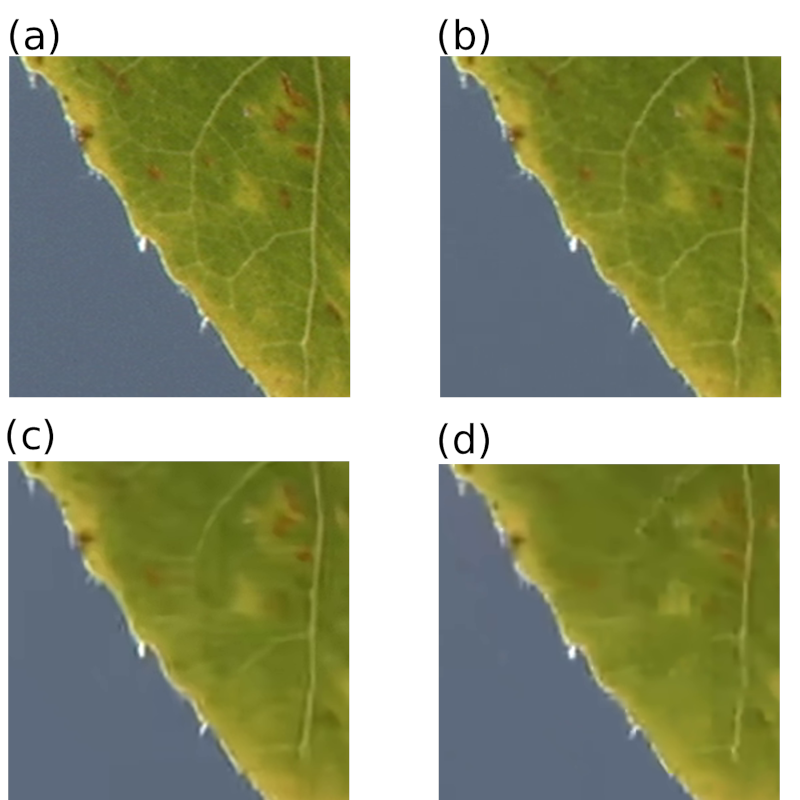
\includegraphics[width=\textwidth]{FIGURES/fig_35.png}
    \caption{Destaque do último quadro do vídeo \textit{aspen\_1080p\_60f} para as sequências (a) original, (b) decodificada pelo VP8, (c) transcodificada original para o AV1 e (d) transcodificada acelerada para o AV1. Fonte: Elaborada pelo autor.}
    \label{fig:35}
\end{figure}


\subsection{Transcodificação Rápida de H.265/HEVC-para-AV1}
\label{cap:7.5.4}

A Tabela \ref{tab:XXXIII} apresenta os resultados obtidos com a transcodificação rápida de H.265/HEVC para AV1, cujo algoritmo foi desenvolvido seguindo a mesma metodologia da proposta de VP9 para AV1. Nesta tabela, é possível observar que a solução é capaz de atingir uma aceleração da transcodificação de 28,36\%, a um custo de 6,74\% de BD-rate. A sequência de maior destaque é \textit{ducks\_take\_off\_1080p50\_60f}, com 41,64\% de TS e 4,10\% de BD-rate. Assim como os resultados de H.264/AVC e de VP8, na proposta para o H.265/HEVC observa-se uma maior redução de tempo nas sequências HD720 do que nas sequências HD1080, para os quais os modelos foram treinados. O fato de só haver uma única sequência HD720 que é caso destacadamente negativa (\textit{dark720p\_120f}), contra os cinco exemplos da resolução HD1080 (\textit{Netflix\_Aerial\_1920x1080\_60fps\_8bit\_420\_60f}, \textit{Netflix\_Crosswalk\_1920x1080\_60fps\_8bit\_420\_60f}, \textit{Netflix\_FoodMarket\_1920x1080\_60fps\_8bit\_420\_60f}, \textit{pedestrian\_area\_1080p25\_60f} e \textit{station2\_1080p25\_60f}) conta bastante para essa diferença em favor da resolução menor, mesmo que pequena. Outro ponto de destaque na proposta de H.265/HEVC para AV1 é que, diferentemente do que observamos no transcodificador rápido de VP9 para AV1, os resultados obtidos na transcodificação de vídeos UHD4K não são compostos por casos negativos. Apesar da baixa aceleração obtida, todos possuem valores de BD-rate baixos (menos de 3,2\%). Isso indica que as amostras geradas pelo decodificador H.265/HEVC em vídeos UHD4K fornecem dados mais confiáveis e de maior qualidade que os gerados pelo decodificador VP9.

\begin{center}
{\footnotesize
\begin{longtblr}[
    caption = {Resultados da transcodificação rápida de H.265/HEVC para AV1 baseado em modelos preditivos.},
    label = {tab:XXXIII}
]{
    colspec = {l|p{6cm}|r|r|r},
    hlines,
    row{even} = {gray9},
    cell{23}{1} = {gray9},
    cell{42}{1} = {white},
}
\hline
\textbf{Resolução} & \textbf{Sequência} & \textbf{BD-rate (\%)} & \textbf{TS (\%)} & \textbf{Razão}\\
\SetCell[r=20]{l}HD720 & boat\_hdr\_amazon\_720p & 4,2537 & 13,99 & 0,304\\
 & dark720p\_120f & 5,4006 & 19,44 & 0,278\\
 & FourPeople\_1280x720\_60 & 2,4022 & 7,98 & 0,301\\
 & FourPeople\_1280x720\_60\_120f & 2,3122 & 8,05 & 0,287\\
 & gipsrestat720p\_120f & 2,6988 & 11,76 & 0,229\\
 & Johnny\_1280x720\_60 & 4,0714 & 14,33 & 0,284\\
 & Johnny\_1280x720\_60\_120f & 3,8174 & 15,76 & 0,242\\
 & KristenAndSara\_1280x720\_60 & 3,0265 & 16,69 & 0,181\\
 & KristenAndSara\_1280x720\_60\_120f & 3,0265 & 16,63 & 0,182\\
 & Netflix\_DinnerScene\_1280x720\_60fps \_8bit\_420\_120f & 6,3817 & 27,47 & 0,232\\
 & Netflix\_DrivingPOV\_1280x720\_60fps \_8bit\_420\_120f & 3,0173 & 12,54 & 0,241\\
 & Netflix\_FoodMarket2\_1280x720\_60fps \_8bit\_420\_120f & 2,966 & 8,99 & 0,330\\
 & Netflix\_RollerCoaster\_1280x720\_60fps \_8bit\_420\_120f & 5,7515 & 25,11 & 0,229\\
 & Netflix\_Tango\_1280x720\_60fps\_8bit \_420\_120f & 4,3562 & 8,07 & 0,540\\
 & rain\_hdr\_amazon\_720p & 1,0663 & 7,37 & 0,145\\
 & vidyo1\_720p\_60fps\_120f & 3,2613 & 12,9 & 0,253\\
 & Vidyo3\_1280x720\_60 & 3,8858 & 14,11 & 0,275\\
 & vidyo3\_720p\_60fps\_120f & 3,6996 & 14,16 & 0,261\\
 & Vidyo4\_1280x720\_60 & 2,9377 & 13,09 & 0,225\\
 & vidyo4\_720p\_60fps\_120f & 3,1043 & 12,99 & 0,239\\
\SetCell[c=2]{r}\textbf{Média dos vídeos HD720} && \textbf{3,5718} & \textbf{14,07} & \\
\SetCell[r=4]{l}HD1080 & aspen\_1080p\_60f & 5,7618 & 9,11 & 0,632\\
 & crowd\_run\_1080p50\_60f & 2,736 & 36,81 & 0,074\\
 & ducks\_take\_off\_1080p50\_60f & 4,4386 & 37,35 & 0,119\\
 & guitar\_hdr\_amazon\_1080p & 6,3438 & 51,96 & 0,122\\
\SetCell[r=14]{l}HD1080 & Netflix\_Aerial\_1920x1080\_60fps\_8bit \_420\_60f & 4,2699 & 29,04 & 0,147\\
 & Netflix\_Boat\_1920x1080\_60fps\_8bit \_420\_60f & 1,7737 & 18,42 & 0,096\\
 & Netflix\_Crosswalk\_1920x1080\_60fps \_8bit\_420\_60f & 3,7432 & 24,88 & 0,150\\
 & Netflix\_FoodMarket\_1920x1080\_60fps \_8bit\_420\_60f & 4,862 & 12,47 & 0,390\\
 & Netflix\_PierSeaside\_1920x1080\_60fps \_8bit\_420\_60f & 3,9322 & 9,41 & 0,418\\
 & Netflix\_SquareAndTimelapse\_1920x 1080\_60fps\_8bit\_420\_60f & 3,7862 & 8,64 & 0,438\\
 & Netflix\_TunnelFlag\_1920x1080\_60fps \_8bit\_420\_60f & 7,6284 & 28,33 & 0,269\\
 & old\_town\_cross\_1080p50\_60f & 7,6534 & 16,34 & 0,468\\
 & park\_joy\_1080p50\_60f & 2,012 & 9,3 & 0,216\\
 & pedestrian\_area\_1080p25\_60f & 4,2314 & 9,42 & 0,449\\
 & rush\_field\_cuts\_1080p\_60f & 2,4349 & 14,08 & 0,173\\
 & rush\_hour\_1080p25\_60f & 4,5744 & 11,41 & 0,401\\
 & seaplane\_hdr\_amazon\_1080p & 3,1675 & 14,68 & 0,216\\
 & station2\_1080p25\_60f & 7,2066 & 10,69 & 0,674\\
\SetCell[c=2]{r}\textbf{Média dos vídeos HD1080} && \textbf{4,4753} & \textbf{19,58} & \\
\SetCell[r=3]{l}UHD4K & Netflix\_BarScene\_4096x2160\_60fps \_10bit\_420\_60f & 3,2829 & 15,88 & 0,207 \\
 & Netflix\_BoxingPractice\_4096x2160 \_60fps\_10bit\_420\_60f & 0,6495 & 11,07 & 0,059\\
 & Netflix\_Dancers\_4096x2160\_60fps \_10bit\_420\_60f & 1,6817 & 11,30 & 0,149\\
\SetCell[c=2]{r}\textbf{Média dos vídeos UHD4K} && \textbf{1,8714} & \textbf{12,75} & \\
\SetCell[c=2]{r}\textbf{Média Geral} && \textbf{6,7454} & \textbf{28,36} & \\
\SetCell[c=2]{r}\textbf{Desvio Padrão Geral} && \textbf{5,0544} & \textbf{15,90} & \\
\hline
\end{longtblr}
}
\end{center}



Há sete sequências que atingem um TS superior à 50\%, sendo que o de maior aceleração dentre eles é o \textit{Netflix\_RollerCoaster\_1280x720\_60fps\_8bit\_420\_120f}, com 55,26\% de TS. No entanto, todos possuem um BD-rate elevado, de aproximadamente 10\%. Por outro lado, a sequência \textit{seaplane\_hdr\_amazon\_1080p} é a que apresenta o menor BD-rate, com apenas 0,02\%. No entanto, também é a sequência com o menor TS de todo o conjunto de vídeos (0,47\%). Inclusive, quase todos os resultados obtidos com a solução H.265/HEVC para AV1 são próximos dos obtidos com a solução H.264/AVC para AV1, variando entre 2\% de BD-rate, para mais ou para menos. Há exceções (13 de 38 sequências, para ser preciso), cujos os dois maiores destaques são para \textit{dark720p\_120f}, que apresenta 15,33\% de BD-rate e 21,91\% de TS no H.265/HEVC contra os 9,15\% e 42,26\% no H.264/AVC; e a sequência \textit{old\_town\_cross\_1080p50\_60f} que obteve 14,05\% de BD-rate e 33,27\% de TS contra os 6,33\% de BD-rate e 21,54\% de TS. 

Não foi encontrado nenhuma relação entre os casos excepcionais que justificasse essa diferença nos resultados, assim como outra relação observada na Tabela \ref{tab:XXXIII}, de que todas as sequências HD1080 com 10 bits de profundidade (HDR) obtiveram um BD-rate inferior a 1\% e, ao mesmo tempo, são os vídeos com menor taxa de aceleração observada.

Há, na literatura científica, outros trabalhos que propõem soluções de transcodificação rápida de H.265/HEVC para AV1, os quais já foram apresentados na seção \ref{cap:6.1}. Além da nossa proposta desenvolvida na seção \ref{cap:6.1}, que apresenta resultados desde TS acima de 50\% ($La$:$Lb$ de 0:0, com 61,20\% de TS e 14,66\% de BD-rate) até menos de 5\% (por exemplo, $La$:$Lb$ de 4:2, com 4,60\% de TS e 0,0583\% de BD-rate), há o trabalho de \citet{bib:chen_2019}, com resultados de redução de TS em 37,8\% a um custo de 0,79\% do BD-rate. Apesar do resultado médio de TS observado na Tabela \ref{tab:XXXIII}, de 28,36\%, ser próximo ao do trabalho de \citet{bib:chen_2019}, inclusive com algumas sequências se aproximando da Razão apresentada por \citeauthor{bib:chen_2019} (de 0,021 pontos), no entanto, o BD-rate apresentado pelo nosso modelo é em ordens de grandeza diferentes.

Observa-se com a comparação da nossa proposta baseada em modelos preditivos com a proposta baseada em heurística, que os resultados médios se aproximam dos observados para a combinação $La$:$Lb$ iguais à 0:1, que apresenta um TS de 32\% e um BD-rate de 6,16\%. Ou senão, avaliando as razões de $La$:$Lb$, a solução proposta neste capítulo se aproxima dos resultados obtidos pelas combinações 0:3 (TS de 15,40\% e BD-rate de 3,58\%), 0:4 (TS de 15,10\% e BD-rate de 3,51\%) e 0:0 (TS de 61,20\% e BD-rate de 14,66\%), contudo, com resultados proporcionalmente melhores.

\subsection{Transcodificação Rápida de H.266/VVC-para-AV1}
\label{cap:7.5.5}

O formato de codificação de vídeo H.266/VVC é sucessor direto dos formatos H.265/HEVC e H.264/AVC. Assim sendo, espera-se observar resultados de redução de tempo similares. No entanto, ao observar os resultados de transcodificação na Tabela \ref{tab:XXXV}, notamos uma aceleração de apenas 12,05\%, mas acompanhado de uma redução considerável no impacto da eficiência de codificação, em relação às outras propostas apresentadas nesta tese, de apenas 1,67\% de BD-rate. O maior BD-rate foi atingido pela sequência \textit{dark720p\_120f}, com 6,12\%, que também apresenta a segunda maior aceleração da transcodificação de H.266/VVC para AV1, de 28,20\%.

\begin{table}
\begin{center}
\caption{Resultados HD1080 da transcodificação rápida de H.266/VVC para AV1 baseado em modelos preditivos.}
\label{tab:XXXV}
\footnotesize

\begin{tblr}{
    colspec = {l|p{6cm}|r|r|r},
    hlines,
    row{even} = {gray9}
}
\hline
\textbf{Resolução} & \textbf{Sequência} & \textbf{BD-rate (\%)} & \textbf{TS (\%)} & \textbf{Razão}\\
\SetCell[r=10]{c}1280$\times$720 & boat\_hdr\_amazon\_720p & 0,3002 & 5,42 & 0,055\\
& dark720p\_120f & 6,1287 & 28,20 & 0,217\\
& FourPeople\_1280x720\_60 & 1,1114 & 7,08 & 0,157\\
& Johnny\_1280x720\_60 & 1,9670 & 10,66 & 0,185\\
& Johnny\_1280x720\_60\_120f & 1,5881 & 33,49 & 0,047\\
& KristenAndSara\_1280x720\_60 & 1,0139 & 9,65 & 0,105\\
& Netflix\_DinnerScene\_1280x720\_60fps \_8bit\_420\_120f & 2,7381 & 2,38 & 1,152\\
& Netflix\_RollerCoaster\_1280x720\_60fps \_8bit\_420\_120f & 1,8403 & 14,84 & 0,124\\
& Netflix\_Tango\_1280x720\_60fps\_8bit \_420\_120f & 1,7705 & 10,73 & 0,165\\
& Vidyo4\_1280x720\_60 & 1,2974 & 11,59 & 0,112\\
\SetCell[c=2]{r}\textbf{Média dos vídeos HD720} && \textbf{1,9756} & \textbf{13,40} & \\
\SetCell[r=16]{c}1920$\times$1080 & aspen\_1080p\_60f & 4,0270 & 18,02 & 0,224\\
& crowd\_run\_1080p50\_60f & 0,4774 & 6,63 & 0,072\\
& ducks\_take\_off\_1080p50\_60f & 1,9142 & 22,52 & 0,085\\
& guitar\_hdr\_amazon\_1080p & 0,2210 & 0,74 & 0,300\\
& Netflix\_Boat\_1920x1080\_60fps\_8bit \_420\_60f & 0,4828 & 8,62 & 0,056\\
& Netflix\_Crosswalk\_1920x1080\_60fps \_8bit\_420\_60f & 2,0820 & 6,65 & 0,313\\
& Netflix\_FoodMarket\_1920x1080\_60fps \_8bit\_420\_60f & 2,7500 & 8,51 & 0,323\\
& Netflix\_PierSeaside\_1920x1080\_60fps \_8bit\_420\_60f & 1,6240 & 12,73 & 0,128\\
& Netflix\_SquareAndTimelapse\_1920x 1080\_60fps\_8bit\_420\_60f & 0,8282 & 7,96 & 0,104\\
& Netflix\_TunnelFlag\_1920x1080\_60fps \_8bit\_420\_60f & 2,1780 & 20,67 & 0,105\\
& pan\_hdr\_amazon\_1080p & 0,2280 & 0,05 & 4,367\\
& park\_joy\_1080p50\_60f & 0,3980 & 13,85 & 0,029\\
& pedestrian\_area\_1080p25\_60f & 2,4390 & 7,35 & 0,332\\
& rush\_field\_cuts\_1080p\_60f & 0,6430 & 16,46 & 0,039\\
& rush\_hour\_1080p25\_60f & 3,4070 & 25,63 & 0,133\\
& seaplane\_hdr\_amazon\_1080p & 0,1260 & 2,93 & 0,043\\
\SetCell[c=2]{r}\textbf{Média dos vídeos HD1080} && \textbf{1,4891} & \textbf{11,21} & \\
\SetCell[c=2]{r}\textbf{Média Geral} && \textbf{1,6762} & \textbf{12,05} & \\
\SetCell[c=2]{r}\textbf{Desvio Padrão Geral} && \textbf{1,3785} & \textbf{8,49} & \\
\hline
\end{tblr}
\end{center}
\end{table}


Apesar da média de aceleração obtida pela transcodificação H.266/VVC para AV1 ser a menor, principalmente em relação aos padrões antecessores do H.266/VVC, o qual se esperava uma aceleração similar, o BD-rate obtido também foi o menor de todos os cinco transcodificadores propostos baseados em aprendizado de máquina. Observe que o \textit{F1-Score} médio dos modelos deste transcodificador (H.266/VVC para AV1) são os menores em relação a todos apresentados na Tabela \ref{tab:XXVI} e, mesmo assim, o BD-rate obtido pelo transcodificador é o menor de todos.

Não há na literatura científica um trabalho de transcodificação rápida de H.266/VVC para AV1, e apesar de haver outros trabalhos de transcodificadores rápidos com os antecessores do H.266/VVC, não é válido utilizá-los como comparação direta. Dos trabalhos existentes na literatura, apenas \citet{bib:lucas_2020} também utiliza o H.266/VVC, mas propondo uma transcodificação rápida de H.265/HEVC para H.266/VVC. Ou seja, \citet{bib:lucas_2020} propõe utilizar o H.266/VVC como formato destino; em contrapartida, nós propomos que o formato H.266/VVC seja o formato de origem. \cite{bib:lucas_2020} propõe utilizar um modelo treinado pelo algoritmo Naïve-Bayes para acelerar o particionamento de blocos 128$\times$128. Com isso, observa-se uma aceleração de 13,38\%, a um custo na eficiência de codificação de 0,32\% de BD-rate. Observa-se que ambas as propostas, a nossa e a de \citet{bib:lucas_2020}, apresentam baixos valores de TS e BD-rate.

Todavia, assim como destacamos sobre comparações entre as soluções propostas com a média observada na literatura, é importante ressaltar que não é possível realizar uma comparação direta entre a proposta de \citet{bib:lucas_2020} à solução apresentada nesta tese, pois são propostas baseadas em diferentes padrões e implementações de codificadores.

\subsection{Considerações Gerais e Análise do \textit{Pipeline} de Processamento}
\label{cap:7.5.6}

Nas subseções anteriores apresentamos todas as cinco propostas de transcodificador rápido usando modelos preditivos, sendo que o \textit{pipeline} de processamento foi desenvolvido para a geração de modelos para o transcodificador de VP9 para AV1 e depois adaptando para gerar modelos para outros transcodificadores com diferentes formatos de origem: H.264/AVC, VP8, H.265/HEVC e H.266/VVC. Tendo como base as mesmas sequências utilizadas para geração dos dados de treinamento e teste, vimos que o \textit{F1-Score} médio dos 12 modelos tende a superar os 0,96 pontos. Considerando algumas limitações de cada experimento, foram disponibilizadas as mesmas sequências para uso na fase preditiva dos modelos, o que possibilitou a geração dos dados comparativos entre o transcodificador original e a proposta de transcodificador rápido. No entanto, houve diferenças de sequências finalizadas em cada uma das propostas. Visando possibilitar uma comparação mais justa entre as cinco propostas de transcodificador rápido baseado em modelos preditivos, a Tabela \ref{tab:XXXVI} apresenta uma visão geral das cinco propostas, contudo, considerando as mesmas sequências de vídeo que estão presente em todas elas.

\afterpage{
\clearpage

\begin{landscape}
\begin{center}
{\footnotesize
\begin{longtblr}[
 caption = {Resumo dos resultados das propostas de transcodificadores rápidos para o formato AV1.},
 label = {tab:XXXVI}
]{ 
 colspec = {lp{5.5cm}|rrrrrrrrrr},
 rowhead = 2,
 hlines,
 row{even} = {gray9},
 cell{3}{1} = {gray9},
 cell{17}{1} = {gray9}
}
\hline
\SetCell[r=2]{c} & \SetCell[r=2]{c}\textbf{Sequência} & \SetCell[c=2]{c}\textbf{VP9} && \SetCell[c=2]{c}\textbf{H.264/AVC} && \SetCell[c=2]{c}\textbf{VP8} && \SetCell[c=2]{c}\textbf{H.265/HEVC} && \SetCell[c=2]{c}\textbf{H.266/VVC} \\
& & BD-rate (\%) & TS (\%) & BD-rate (\%) & TS (\%) & BD-rate (\%) & TS (\%) & BD-rate (\%) & TS (\%) & BD-rate (\%) & TS (\%) \\
\SetCell[r=9]{c}\rotatebox[origin=c]{90}{1280$\times$720} & dark720p\_120f & 5,40 & 19,44 & 9,16 & 42,26 & 23,12 & 76,25 & 15,33 & 21,91 & 6,13 & 28,20 \\
& FourPeople\_1280x720\_60 & 2,40 & 7,98 & 2,63 & 32,32 & 6,41 & 71,03 & 3,40 & 16,54 & 1,11 & 7,08 \\
& Johnny\_1280x720\_60 & 4,07 & 14,33 & 7,74 & 48,34 & 16,25 & 79,12 & 9,71 & 55,15 & 1,97 & 10,66 \\
& Johnny\_1280x720\_60\_120f & 3,82 & 15,76 & 8,02 & 49,13 & 16,25 & 79,70 & 9,04 & 52,35 & 1,59 & 33,49 \\
& KristenAndSara\_1280x720\_60 & 3,03 & 16,69 & 6,06 & 47,96 & 13,42 & 80,78 & 7,62 & 52,93 & 1,01 & 9,65 \\
& Netflix\_DinnerScene\_1280x720\_ 60fps\_8bit\_420\_120f & 6,38 & 27,47 & 13,09 & 37,94 & 25,67 & 62,58 & 14,35 & 47,47 & 2,74 & 2,38 \\
& Netflix\_RollerCoaster\_1280x720\_ 60fps\_8bit\_420\_120f & 5,75 & 25,11 & 6,79 & 43,18 & 15,33 & 66,61 & 11,35 & 55,26 & 1,84 & 14,84 \\
& Netflix\_Tango\_1280x720\_60fps\_8bit \_420\_120f & 4,36 & 8,07 & 4,37 & 9,20 & 7,52 & 21,39 & 5,58 & 10,46 & 1,77 & 10,73 \\
& Vidyo4\_1280x720\_60 & 2,94 & 13,09 & 9,14 & 48,11 & 16,25 & 76,42 & 8,80 & 48,99 & 1,30 & 11,59 \\
\SetCell[c=2]{c}\textbf{Média HD720} && \textbf{4,24} & \textbf{16,44} & \textbf{7,45} & \textbf{39,83} & \textbf{15,58} & \textbf{68,21} & \textbf{9,47} & \textbf{40,12} & \textbf{2,16} & \textbf{14,29} \\
\SetCell[r=5]{c}\rotatebox[origin=c]{90}{1920$\times$1080} & aspen\_1080p\_60f & 5,76 & 9,11 & 15,15 & 33,99 & 24,20 & 29,86 & 19,49 & 52,30 & 4,03 & 18,02 \\
& crowd\_run\_1080p50\_60f & 2,74 & 36,81 & 0,89 & 15,65 & 1,55 & 30,57 & 1,27 & 25,93 & 0,48 & 6,63 \\
& ducks\_take\_off\_1080p50\_60f & 4,44 & 37,35 & 3,36 & 25,83 & 4,49 & 49,62 & 4,11 & 41,64 & 1,91 & 22,52 \\
& Netflix\_Boat\_1920x1080\_60fps\_8bit \_420\_60f & 1,77 & 18,42 & 1,88 & 20,37 & 2,83 & 31,87 & 1,96 & 23,41 & 0,48 & 8,62 \\
& Netflix\_Crosswalk\_1920x1080\_60fps \_8bit\_420\_60f & 3,74 & 24,88 & 10,34 & 12,52 & 23,16 & 32,74 & 9,48 & 20,96 & 2,08 & 6,65 \\
\SetCell[r=8]{c}\rotatebox[origin=c]{90}{1920$\times$1080}& Netflix\_FoodMarket\_1920x1080\_ 60fps\_8bit\_420\_60f & 4,86 & 12,47 & 9,51 & 19,58 & 16,08 & 32,88 & 12,53 & 25,21 & 2,75 & 8,51 \\
& Netflix\_PierSeaside\_1920x1080\_ 60fps\_8bit\_420\_60f & 3,93 & 9,41 & 11,05 & 41,32 & 14,27 & 76,93 & 6,95 & 45,00 & 1,62 & 12,73 \\
& Netflix\_SquareAndTimelapse\_1920x 1080\_60fps\_8bit\_420\_60f & 3,79 & 8,64 & 3,05 & 12,59 & 4,92 & 26,52 & 3,80 & 17,14 & 0,83 & 7,96 \\
& Netflix\_TunnelFlag\_1920x1080\_ 60fps\_8bit\_420\_60f & 7,63 & 28,33 & 6,77 & 17,90 & 11,58 & 33,64 & 12,46 & 56,71 & 2,18 & 20,67 \\
& park\_joy\_1080p50\_60f & 2,01 & 9,30 & 1,02 & 12,37 & 2,22 & 54,74 & 1,10 & 18,89 & 0,40 & 13,85 \\
& pedestrian\_area\_1080p25\_60f & 4,23 & 9,42 & 8,18 & 14,23 & 22,98 & 72,67 & 9,28 & 20,36 & 2,44 & 7,35 \\
& rush\_field\_cuts\_1080p\_60f & 2,43 & 14,08 & 1,06 & 13,72 & 1,92 & 30,92 & 1,57 & 26,62 & 0,64 & 16,46 \\
& rush\_hour\_1080p25\_60f & 4,57 & 11,41 & 8,48 & 14,01 & 22,39 & 75,96 & 9,09 & 23,93 & 3,41 & 25,63 \\
\SetCell[c=2]{c}\textbf{Média HD1080} && \textbf{3,99} & \textbf{17,66} & \textbf{6,21} & \textbf{19,54} & \textbf{11,74} & \textbf{44,53} & \textbf{7,16} & \textbf{30,62} & \textbf{1,79} & \textbf{13,51} \\
\SetCell[c=2]{c}\textbf{Média Geral} && \textbf{4,09} & \textbf{17,16} & \textbf{6,72} & \textbf{27,84} & \textbf{13,31} & \textbf{54,22} & \textbf{8,10} & \textbf{34,51} & \textbf{1,94} & \textbf{13,83} \\
\SetCell[c=2]{c}\textbf{Desvio Padrão Geral} && \textbf{1,48} & \textbf{9,08} & \textbf{4,03} & \textbf{14,61} & \textbf{8,20} & \textbf{22,03} & \textbf{4,97} & \textbf{15,90} & \textbf{1,34} & \textbf{7,97}\\
\SetCell[c=2]{c}\textbf{Razão Geral das Médias} && \SetCell[c=2]{c}\textbf{0,238} && \SetCell[c=2]{c}\textbf{0,241} && \SetCell[c=2]{c}\textbf{0,245} && \SetCell[c=2]{c}\textbf{0,235} && \SetCell[c=2]{c}\textbf{0,140} &\\
\hline
\end{longtblr}
}
\end{center}
\end{landscape}
}



Algumas observações imediatas são possíveis a partir da Tabela \ref{tab:XXXVI}. A primeira delas é a quantidade de sequências levemente inferior ao apresentado nas subseções anteriores. Mesmo assim, foram transcodificadas em todas as cinco propostas, nove na resolução HD720 e 13 na resolução HD1080. Considerando que os artigos existentes na literatura tendem a apresentar quatro sequências por resolução, então é possível afirmar que a confiabilidade dos resultados médios apresentados na Tabela \ref{tab:XXXVI} é superior ao usualmente aplicado na literatura. Outra observação possível é que a aceleração média atingida pelas propostas realizadas varia entre 13,83\% (de H.266/VVC para AV1) até 54,22\% (de VP8 para AV1), a um custo de impactar na eficiência de codificação desde 13,31\% (de VP8 para AV1) até apenas 1.94\% (de H.266/VVC para AV1). Com isso, é possível identificar os transcodificadores com resultados extremos, com a proposta de VP8 para AV1 sendo a que apresenta a maior Razão média, de 0,245, e a proposta de H.266/VVC para AV1 com a menor Razão média, de 0,140. Considerando que as outras três propostas apresentam uma Razão média com valores próximos ao observado na proposta de VP8 para AV1, é possível afirmar, então, que a proposta de transcodificador rápido de H.266/VVC para AV1 usando modelos preditivos é a que apresenta os melhores resultados nesta tese.

Avaliando os resultados que geraram a Tabela \ref{tab:XXXVI}, em especial na resolução HD1080 que é a resolução utilizada para treinamento dos modelos, é possível identificar quais sequências foram consistentes em apresentar os melhores resultados, sendo elas: \textit{crowd\_run\_1080p50\_60f}, \textit{rush\_field\_cuts\_1080p\_60f} e \textit{Netflix\_Boat\_1920x1080\_60fps\_8bit\_420\_60f}, que apresentaram uma média de aceleração, respectivamente, de 23,12\%, 20,36\% e 20,54\% a um custo de 1,39\%, 1,52\% e 1,79\% de BD-rate. Ou seja, foram sequências que apresentaram uma boa aceleração com baixo impacto na eficiência de codificação. Essas três sequências com resultados positivos apresentam boa quantidade de elementos em movimento em cenas distantes. Por outro lado, as três sequências com maior consistência negativa foram \textit{aspen\_1080p\_60f}, \textit{Netflix\_Crosswalk\_1920x1080\_60fps\_8bit\_420\_60f} e \textit{Netflix\_FoodMarket\_1920x1080\_60fps\_8bit\_420\_60f}, apresentando respectivamente valores médios de BD-rate de 13,73\%, 9,76\% e 9,15\%, acompanhados de uma aceleração média de 28,66\%, 19,55\% e 19,73\%. Ou seja, apesar dos valores de aceleração serem positivos para um objetivo de transcodificação rápida, os valores de BD-rate gerados nestas sequências são muito elevados, ainda mais considerando-se a média observada na literatura. A principal similaridade entre essas três sequências é a presença de movimento com texturas finas. Nas Figuras \ref{fig:36} e \ref{fig:37}, mostramos o primeiro quadro sem compressão dessas seis sequências.

\afterpage{
\clearpage
\begin{landscape}
\begin{figure}
    \centering
    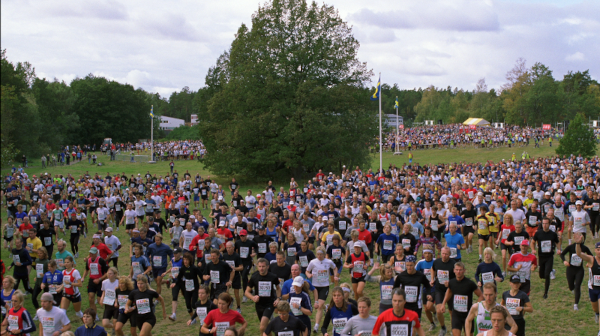
\includegraphics[height=0.4\textheight]{FIGURES/fig_36_1.png}
    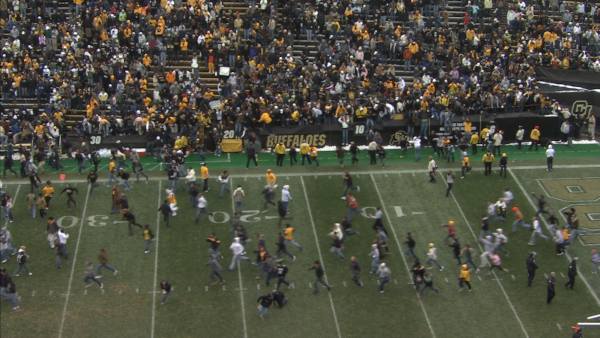
\includegraphics[height=0.4\textheight]{FIGURES/fig_36_2.png}
    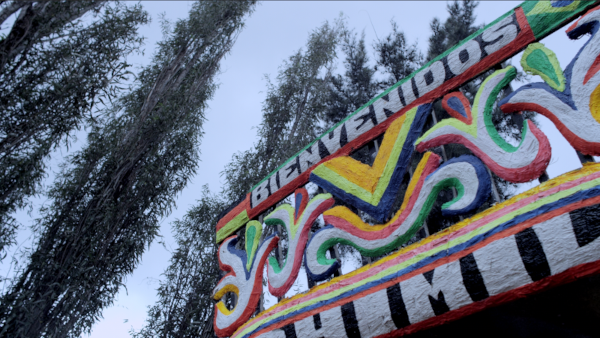
\includegraphics[height=0.4\textheight]{FIGURES/fig_36_3.png}
    \caption{Primeiro quadro das sequências HD1080 de maior destaque positivo em todos os experimentos, acima \textit{crowd\_run\_1080p50\_60f}, no meio \textit{rush\_field\_cuts\_1080p\_60f} e abaixo \textit{Netflix\_Boat\_1920x1080\_60fps\_8bit\_420\_60f}. Fonte: Elaborada pelo autor.}
    \label{fig:36}
\end{figure}
\end{landscape}
}

Desta forma, considerando tudo o que já foi abordado até o momento, é possível concluir que há sequências de vídeos em que as propostas de transcodificadores rápidos desenvolvidas apresentam resultados de redução de complexidade e impacto na eficiência de codificação dentro de valores desejáveis, como pode ser visto na Tabela \ref{tab:XXXVI}. Inclusive, as sequências com os resultados negativos nos mostram que há uma fragilidade na precisão do modelo implementado. Como apontado anteriormente, o uso da técnica de balanceamento de dados \textit{undersampling} aplica uma redução da capacidade de discernimento no limite entre decisões binárias. Desta forma, é preciso investigar e avaliar os melhores balanceamentos dos conjuntos de dados utilizados para treinamento e teste dos modelos, de forma a reduzir essa imprecisão entre particionar ou não particionar.

\afterpage{
\clearpage
\begin{landscape}
\begin{figure}
    \centering
    
\includegraphics[height=0.4\textheight]{FIGURES/fig_37_1.png}
    
\includegraphics[height=0.4\textheight]{FIGURES/fig_37_2.png}
    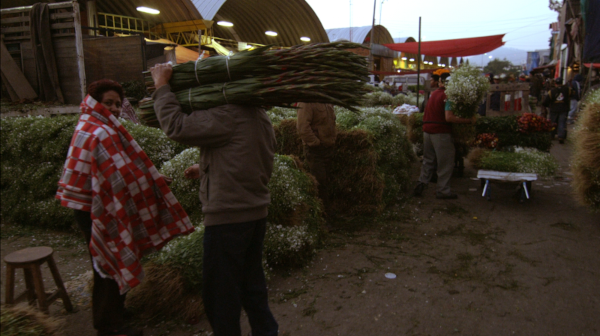
\includegraphics[height=0.4\textheight]{FIGURES/fig_37_3.png}
    \caption{Primeiro quadro das sequências HD1080 de maior destaque negativo em todos os experimentos, acima \textit{aspen\_1080p\_60f}, no meio \textit{Netflix\_Crosswalk\_1920x1080\_60fps\_8bit\_420\_60f} e abaixo \textit{Netflix\_FoodMarket\_1920x1080\_60fps\_8bit\_420\_60f}. Fonte: Elaborada pelo autor.}
    \label{fig:37}
\end{figure}
\end{landscape}
}

